\documentclass[12pt,oneside]{book}
\usepackage[spanish]{babel}
\usepackage[utf8]{inputenc}
\pagestyle{plain}
\usepackage{graphicx}
\usepackage{makeidx}
\usepackage{enumitem}
\usepackage{amsmath}
\usepackage{amsfonts}
%\usepackage{nomencl}


\textheight=235mm
\textwidth=145mm
\topmargin=0mm
\headheight=0mm
\headsep=0mm

% These must be changed for double sided output !

\oddsidemargin=15mm
\evensidemargin=15mm

\makeindex
\makeglossary
\begin{document}

% set line spacing to 1.5B
\baselineskip = 17pt


\title{ Estimación de la mirada}
\author{Rajiv Raciel González González}
\date{2017}
\maketitle 
\frontmatter

\chapter{Resumen}


\tableofcontents

% Contents not put in table of contents by default so add it separately

\addcontentsline{toc}{chapter}{Contenidos}


\listoffigures


% List of figures  not put in table of contents by default so add it separately

\addcontentsline{toc}{chapter}{Lista de figuras}


\chapter{Agradecimientos}

CONACYT

%\printglossary

\addcontentsline{toc}{chapter}{Nomenclatura}


\mainmatter

\chapter{Objetivos}
\section{Objetivo general}

Detectar el rostro de las personas y estimar su pose relativa a un plano virtual situado enfrente de ellas, asociando regiones en dicho plano con información de textura de los rostros detectados y su posición. 
 \section{Objetivos específicos}
   \begin{itemize}
   	\item Generar una base de datos de rostros humanos con la información de
   	pose asociada.
   	\item Desarrollar el sistema para que funcione en un rango de distancia am-
   	plio entre la persona y la cámara.
   	\item Implementación de un algoritmo clasificador para asociar la región que
   	se observa con poses determinadas.
   \end{itemize}
   
   \chapter{Introducción}
   Conocer la posición, orientación y movimiento de la cabeza son cuestiones de gran importancia ya que pueden ayudar a las personas a interactuar con las computadoras de una forma más natural a como se realiza actualmente, dando como resultado en útiles  aplicaciones como: video conferencias, controles o interfaces hombre-máquina especiales, aplicaciones de realidad virtual. Además, si se toma en cuenta hacia dónde está mirando la persona y el tiempo que lleva en cierta posición puede proporcionar información adicional que ayudaría a inferir si está muy atenta a lo que está observando o si la persona está durmiendo.\\
   Por medio del análisis de imágenes capturadas a personas y en combinación con algoritmos de aprendizaje automático es posible conocer la posición y  orientación de sus cabezas con respecto a un marco de referencia, la información obtenida puede ayudar a conocer qué es lo que están observando las personas, lo cual es el objetivo principal del presente trabajo de tesis, estimar la mirada de las personas en un plano enfrente de ellas.
   
   %%%%%%%%%%%%%%%%%%%%%%%%%%%%%%%%%%%%%%%%%%%%%%%%%%%%%%%
   %%%%%%%%%%%%%%%%%%%%%%%%%%%%%%%%%%%%%%%%%%%%%%%%%%%%%%%
   %%%%%%%%%%%%%%%%%%%%%%%%%%%%%%%%%%%%%%%%%%%%%%%%%%%%%%%
\chapter{Marco teórico}

	Para realizar la estimación de la mirada de las personas en un plano virtual enfrente de ellas es necesario saber algunos conceptos, definiciones y algunos conocimientos que sirvan de apoyo al desarrollo del presente trabajo de tesis. En este capítulo se describen las bases para llevar a cabo el proyecto, dichas bases consisten principalmente de visión computacional, geometría proyectiva, algoritmos de aprendizaje supervisado, algoritmos de optimización numérica....

   %Añadir un parrafo de lo que aporta el de nosotros (plano)
   %Tomando en cuenta las consideraciones anteriores 
   %El proyecto de tesis propuesto además de estimar la pose de la cabeza mediante algoritmos de aprendizaje automático utilizará dichos algoritmos para asociarle a las cabezas humanas una región 

   
   \section{Detector de rostros de Viola y Jones}
  Como ya se ha mencionado anteriormente para estimar la mirada con precisión se necesita un sistema de detección y seguimiento de ojos además de múltiples cámaras y el sistema de estimación de pose de la cabeza, habiendo señalado lo anterior cabe destacar que el proyecto que se desarrollará más que estimar la mirada con precisión (además de la pose de la cabeza) representándola como un vector normal al iris,  se pretende estimar una región en un plano virtual enfrente de ellas, la región indicaría lo que están observando las personas de la escena que tienen enfrente. \\
   
   En el presente proyecto para la estimación de la pose de la cabeza de las personas en primer lugar se debe detectar dónde se encuentran los rostros (como se ha mencionado) para luego estimar su pose, ya que el sistema consiste de muchas etapas, se requiere que la detección se haga lo más rápido posible y eficientemente,  por lo tanto se decidió utilizar uno de los algoritmos de detección más utilizados y rápidos que existen: el clasificador basado en características tipo Haar en cascada. Este método fue propuesto por Paul Viola y Michael Jones en 2001 en el artículo Rapid Object Detection using a Boosted Cascade of Simple Features, el método consta principalmente de las siguientes etapas.
   
   \subsection{Imagen integral}
   En esta etapa se utiliza una representación intermedia de la imagen conocida como imagen integral o también conocida como tablas de áreas sumadas [Crow 1984]. En la imagen integral a cada pixel de la imagen se le asocia un valor representando la suma de los valores de los píxeles que se encuentran arriba y a la izquierda de él, así como también se le suma su valor de píxel. Este tipo de representación tiene como principal ventaja la rápida estimación del valor de los píxeles de subregiones de la imagen.
   \begin{figure}[htbp]
   	\centering
   	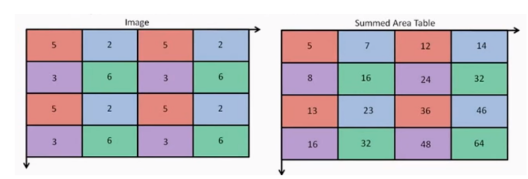
\includegraphics[width=0.7\textwidth]{./pictures/imagenIntegral}
   	\caption{Ejemplo de imagen integral}\label{fig: figura}
   \end{figure}
   El detector de Viola y Jones clasifica las imágenes basado en el valor de simples características, los sistemas basados en características operan muchos más rápido que los basados en píxeles. La imagen integral puede ser usada para estimar el valor de características tipo Haar, las características Haar se visualizan como rectángulos adyacentes blancos y negros, el valor que generan se calcula de la diferencia de la suma de los pixeles en el área blanca menos la suma de los del área negra, la adyacencia que presentan los rectángulos permite reutilizar algunos valores. El conjunto de características rectangulares ofrece una muy buena representación de imágenes la cual soporta un efectivo entrenamiento.
   
   \begin{figure}[htbp]
   	\centering
   	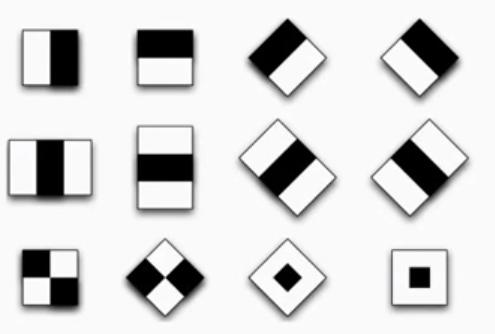
\includegraphics[width=0.4\textwidth]{./pictures/haar}
   	\caption{Características Haar}\label{fig: figura}
   \end{figure}
   
   \subsection{Algoritmo AdaBoost}
   Los métodos de Boosting [Friedman et al 2000] básicamente consisten en combinar la eficiencia de muchos clasificadores débiles para producir un poderoso consejo o comité clasificador. El algoritmo Adaboost es el método más usado y práctico de los algoritmos de Boosting. La idea general del AdaBoost consiste en que los ejemplos que son clasificados erróneamente obtienen mayor peso en las iteraciones siguientes, esto significa que los ejemplos que se encuentran cerca de la frontera de decisión son generalmente más difíciles de clasificar y por lo tanto se les asigna mayores pesos después de unas cuantas iteraciones. La idea de reasignación de pesos en el conjunto de entrenamiento es esencial en los métodos de Boosting.
   El detector de Viola y Jones se entrenó con conjuntos de imágenes etiquetadas como positivas y negativas, el algoritmo de AdaBoost fue utilizado para entrenar al clasificador y seleccionar un conjunto pequeño con las características Haar más importantes de una muy amplia biblioteca de posibles características. Como resultado final del proceso de entrenamiento el algoritmo de AdaBoost produce un clasificador robusto que tiene la forma de un perceptrón, una combinación de clasificadores débiles en el que cada clasificador tiene asociado una sola característica Haar y un umbral. Resumiendo lo anteriormente mencionado, la utilización del algoritmo de clasificación AdaBoost permite encontrar las características que mejor separan los ejemplos positivos de los negativos. Una de las ventajas clave por la cual fue elegido AdaBoost como algoritmo seleccionador de características por Viola y jones en su detector, es la increíble velocidad que presenta; usando AdaBoost, un clasificador de 200 características puede ser construido en alrededor 10-11 operaciones de procesador. Las primeras características seleccionadas por AdaBoost tienen mucho sentido y son fáciles de interpretar, una de esas característica parece enfocarse en la propiedad de que la región de los ojos es por lo regular más oscura que la región de la nariz y las mejillas.
   \begin{figure}[htbp]
   	\centering
   	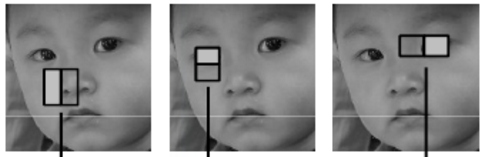
\includegraphics[width=0.7\textwidth]{./pictures/adaboost}
   	\caption{Características tipo Haar sobrepuestas}\label{fig: figura}
   \end{figure}
   
   \subsection{Filtro con estructura en cascada.}
   El último componente importante del Detector de Viola y Jones es la estructura en cascada que se forma con la combinación de unos cuantos clasificadores mejorados (boosted), estos clasificadores son usados para rechazar la mayor??a de las subregiones negativas (sin rostros de personas) y poner atención en regiones de la imagen más prometedoras, es decir, las regiones que presenten el rostro de alguna persona. Este método es muy eficiente ya que la mayor??a de las sub-ventanas o subregiones son rechazadas en etapas tempranas. Se le denominó estructura en ?cascada? debido a la forma que presenta al momento de procesar las sub- ventanas. Las sub-ventanas de la entrada del detector pasan a través de una serie de nodos, cada nodo toma una decisión binaria y dependiendo de la decisión la subregión se mueve al siguiente nodo o se rechaza. El número de clasificadores débiles presentes en cada nodo incrementa conforme la sub-ventana se va moviendo a los siguientes nodos, por ejemplo, en el primer nodo contiene un clasificador débil, el segundo 10, el tercero 25, el cuarto 50 y as?? sucesivamente. Teniendo pocos clasificadores en etapas tempranas es otra forma de mejorar la velocidad del detector y esto de alguna forma compensa el costo de evaluar cada caracter??stica Haar en diferentes escalas y posiciones de la imagen.
   \begin{figure}[htbp]
   	\centering
   	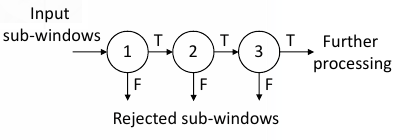
\includegraphics[width=0.7\textwidth]{./pictures/cascada}
   	\caption{Diagrama de nodos}\label{fig: figura}
   \end{figure}
   
   El detector de rostros descrito en esta sección tiene incontables aplicaciones y debido la velocidad de la detección puede ser utilizado en aplicaciones que requieran detección en tiempo real. Uno de los aspectos más interesantes del método de Viola y Jones es que no se limita a la detección de rostros, puede ser modificado para sistemas detectores de otro tipo de patrones en las imágenes, por ejemplo automóviles, peatones y recientemente utilizado para la detección de la enfermedad de Chagas, mediante las muestras de sangre de los infectados [Uc Cetina et al 2015].
   \begin{figure}[htbp]
   	\centering
   	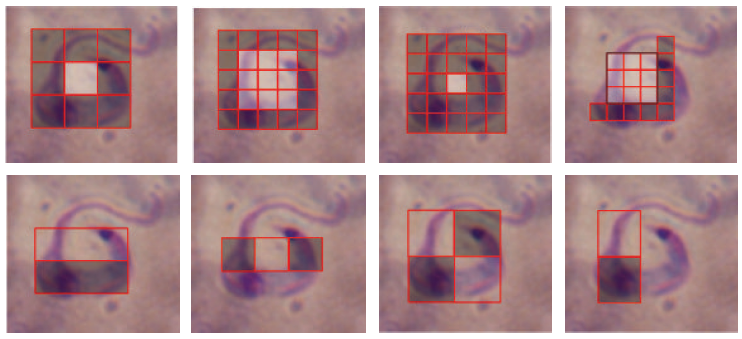
\includegraphics[width=0.7\textwidth]{./pictures/chagas}
   	\caption{Detección de chagas en la sangre mediante el método de Viola y Jones}\label{fig: figura}
   \end{figure}
   
   \section{Matrices de Rotación}
   \section{Homografía}
   \section{Modelo pinhole de cámara}
   \section{Calibración de cámaras y corrección de imágenes}
   \section{Optimización numérica y Levenberg-Marquardt}
   \section{Aprendizaje Automático}
   \section{Redes neuronales artificiales}




\chapter{Metodología}
    \section{Mapeo de coordenadas a ángulos}
    Uno de los problemas que hay que tomar en cuenta y definir en el presente trabajo de tesis antes de realizar los experimentos, es la relación que existe entre la ubicación en metros de lo que está mirando el sujeto de estudio en la pantalla y la pose de la cabeza de esta persona medida en ángulos, tomando en cuenta diversos aspectos como: la estatura de la persona, la distancia de la persona a la pantalla, cuál es el marco de referencia, etc. Esta sección consiste en describir cómo se realiza el mapeo (o la ecuación) de dicho objeto desplegado en pantalla y la orientación de la cabeza, primero se describirá la geometría del escenario. 
    \begin{figure}[htbp]
    	\centering
    	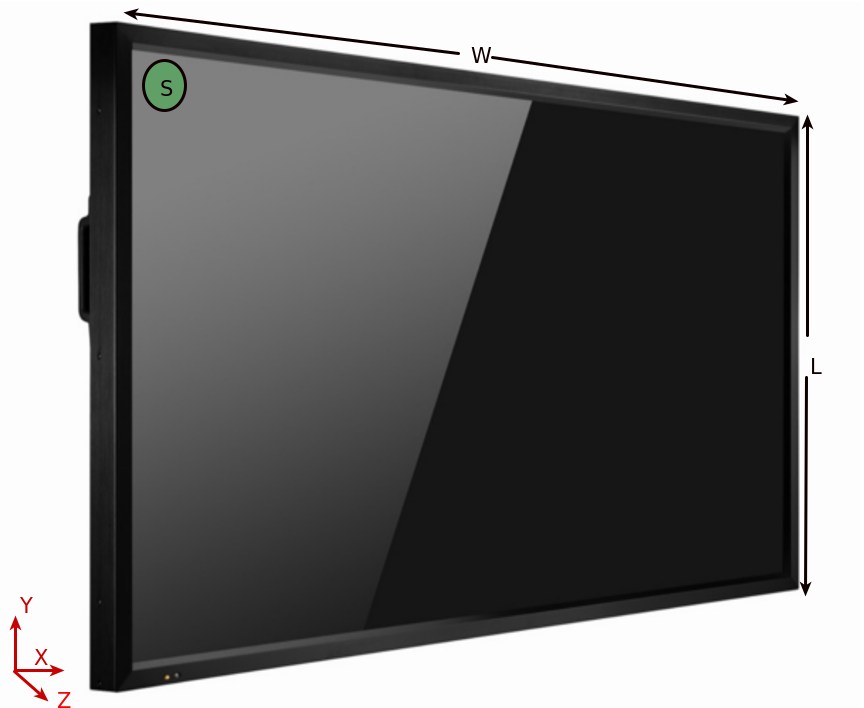
\includegraphics[width=0.5\textwidth]{./pictures/pantalla2}
    	\caption{}\label{fig: figura}
    \end{figure}   
    \\La pantalla que observa el sujeto del experimento se coloca en una pared a una distancia de $L_y$ metros del piso, la pantalla tiene unas dimensiones de $W$ m. de ancho y $L$ m. de alto. El sistema de coordenadas tiene su origen en la cámara y se ubica  encima de la pantalla y a la mitad del ancho W, \textbf{la recta que se encuentra a lo largo de W es paralela al eje $X$ y la que está a lo largo de L es paralela a $Y$}. Las personas se encontrarán paradas en un mismo plano (piso) y enfrente de la pantalla a una distancia $D_z$. Hay un punto en específico del rostro de las personas que es de interés y es el que se utiliza para realizar el análisis, este punto se define como $P$ y se encuentra a la mitad de la linea que une los ojos. El vector $\vec v$ sale del punto $P$ y es ortogonal al plano de la cara, el punto $P$ se encuentra a una distancia $H_y$ con respecto al piso y es dependiente de la estatura de la persona. Otro parámetro que se debe mencionar es el que hace referencia a la distancia que hay entre la persona y el origen sobre el eje $X$, es decir, la componente $X$ del punto $P$ de la persona y lo denotaremos como $a$.%La recta imaginaria que une el punto $P$ con el piso es $L_p$ y es perpendicular al plano del piso y por la misma razón es paralela al eje $Y$.
    \begin{figure}[htbp]
    	\centering
    	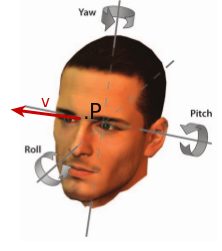
\includegraphics[width=0.36\textwidth]{./pictures/personaMirando}
    	\caption{}\label{fig: figura}
    \end{figure}
    
    Como se puede observar en la figura 1.2 las personas tenemos tres tipos de movimiento de la cabeza: yaw, pitch y roll; sin embargo para el análisis de este proyecto solo se toman en cuenta el movimiento de yaw y pitch, ya que estos son los movimientos que se dan cuando una persona mueve su cabeza para observar el objeto en dos dimensiones de la pantalla.\\
    El objeto de la pantalla que la persona observa es representado como $S$ y el vector $\vec v$ representa la mirada de la persona o lo que es lo mismo $\vec{PS}$, cuando la persona se encuentre mirando $S$ el vector $\vec v$  debe apuntar a $S$, esto quiere decir que si se proyecta el vector sobre la misma dirección hacia la pantalla debe intersectar $S$.\\
    El objeto $S$ se desplazará a través de toda la pantalla $(X,Y)$ metros, tomando como marco de referencia la esquina superior izquierda de la pantalla, a esta esquina le corresponde la coordenada $(0,0)$, $(X,Y)$ es la esquina inferior derecha y $(\frac{X}{2}, \frac{Y}{2})$ el centro de la pantalla.
    La pose de la cabeza se mide mediante dos ángulos: $\phi_x$ y $\phi_y$.
    \begin{itemize}
    	\item $\phi_y$.- Observando desde el plano $Y-Z$ representa que tanto se desvía el vector $\vec v$% sobre la recta $D_z$ que hay entre la persona y la pantalla.
    	\item $\phi_x$.- Observando desde el plano $X-Z$ (desde arriba de la persona y la pantalla) representa que tanto se desvía el vector $\vec v$ %sobre la recta $D_z$.
    \end{itemize}
    De igual manera el ángulo $\phi_x$ indica el movimiento yaw que la persona realiza al mirar como se traslada el objeto $S$ y el ángulo $\phi_y$ el movimiento pitch.
    
    \section{Ecuaciones}
    Una vez definido el escenario y los aspectos a tomar en cuenta, ahora falta demostrar cual es la relación que se puede hallar entre la posición del objeto en la pantalla y la pose de la cabeza mediante los ángulos $\phi_x$ y $\phi_y$.
    
    \subsection{Desviación de $\phi_y$ y $\phi_x$. Primer caso}
    Para facilitar el análisis en esta sección se ilustra el escenario con todos los elementos en la figura 2.1
    \begin{figure}[htbp]
    	\centering
    	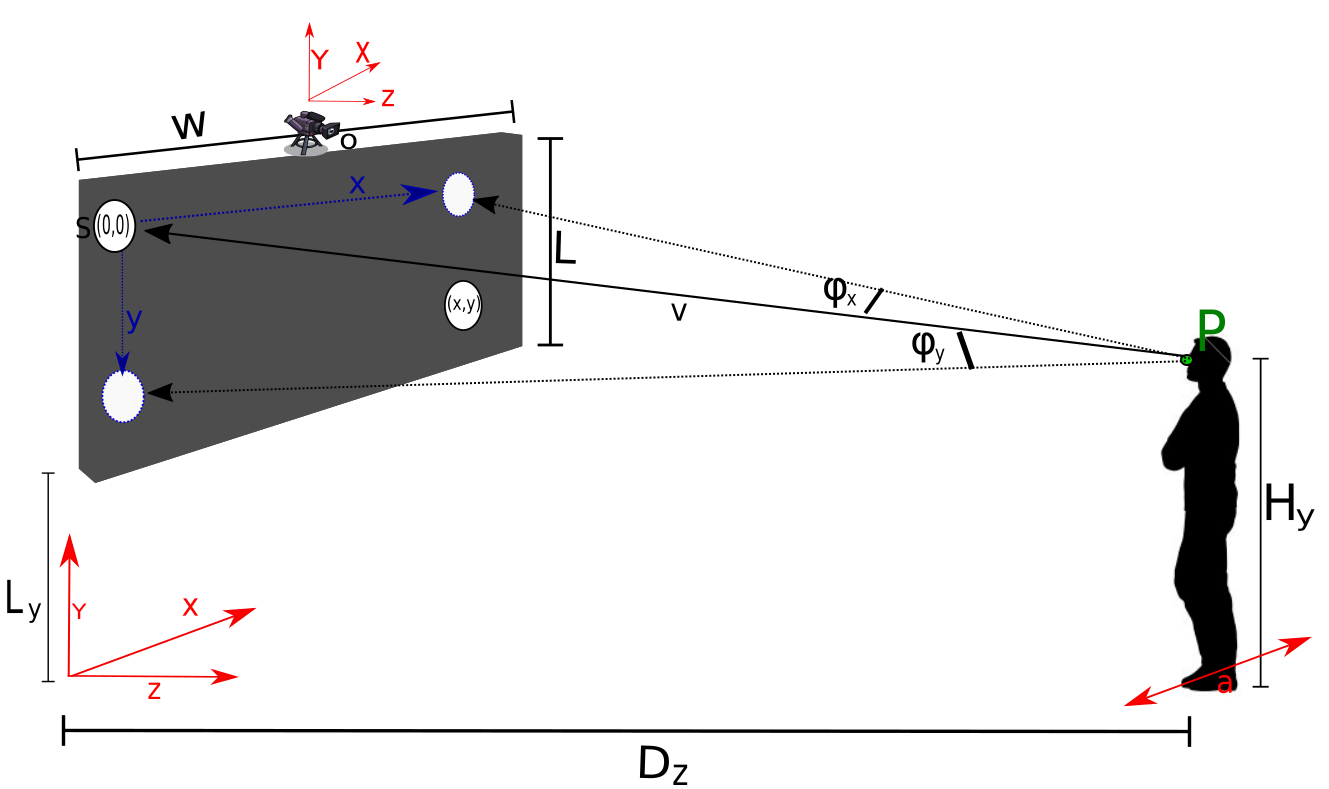
\includegraphics[width=0.7\textwidth]{./pictures/escenario}
    	\caption{Escenario y aspectos a tomar en cuenta}\label{fig: figura}
    \end{figure}
    \\Este caso es suponiendo que la cámara está colocada sobre la pantalla de tal forma que su eje $Z$ es paralelo al piso, esto quiere decir que el eje $Y$ de la cámara yace sobre el plano de la pantalla.\\
     El análisis comienza observando la escena desde el plano $Y-Z$, primero se definen dónde se encuentran con respecto al sistema de coordenadas los puntos más importantes, los cuales son: $S$ y $P$. Supongamos que el objeto a observar está en la coordenada $(x,y)$ de la pantalla, como se había mencionado previamente el sistema de coordenadas se encuentra centrado en la cámara,  a la mitad de la pantalla con respecto al eje $X$ y a una pequeña altura $c_y$ m. con respecto al eje y, el movimiento de $S$ yace sobre el plano $X-Y$ por lo que su componente en $z$ es igual cero, entonces:
    
    \begin{eqnarray}
    S= [S_x, S_y, S_z]^T= [x-W/2, -(c_y+y), 0]^T
    \end{eqnarray}
    Para hallar las componentes de P se toma la distancia $D_z$ a la que se encuentra del origen sobre el eje $Z$, como se había mencionado la persona se desplaza $a$ m sobre el eje $X$ y se encuentra a una distancia sobre el eje y de $L_y+L-H_y$:
    \begin{eqnarray}
    P=[P_x, P_y, P_z]^T= [a, -(L_y+L-H_y), D_z]^T
    \end{eqnarray}
  Ahora que ya se definieron donde se encuentran los puntos que se utilizarán con respecto al marco de referencia centrado en la cámara, se necesitan los ángulos entre la posición del vector $\vec v=\vec {PS}$ y cada uno de los ejes que son de interés, estos ángulos se conocen como cosenos directores del vector $\vec v$ y únicamente son necesarios los que se forman con el eje $Y$ y el $X$.
  Las fórmulas de los cosenos directores son:
  \begin{eqnarray}
  cos(\phi_y)=\frac{\vec v_y}{|\vec v|}\\
  cos(\phi_x)=\frac{\vec v_x}{|\vec v|}
  \end{eqnarray}
  
  donde $|\vec v|$ se halla mediante:
  \begin{eqnarray}
  \sqrt{\vec v_{x}^2+\vec v_{y}^2+\vec v_{z}^2}=\sqrt{(x-\frac{W}{2}-a)^2+(-c_y-y+(L_y+L-H_y))^2+(-D_z)^2}
  \end{eqnarray}
  \\Por lo tanto los ángulos de desviación son:
  
  \begin{eqnarray}
  \phi_y=cos^{-1} (\frac{-c_y-y+(L_y+L-H_y)}{\sqrt{(x-\frac{W}{2}-a)^2+(-c_y-y+(L_y+L-H_y))^2+(-D_z)^2}})\\
  \phi_x=cos^{-1}(\frac{x-\frac{W}{2}-a}{\sqrt{(x-\frac{W}{2}-a)^2+(-c_y-y+(L_y+L-H_y))^2+(-D_z)^2}})
  \end{eqnarray}
   \subsubsection{Análisis del comportamiento de los ángulos $\phi_x$ y $\phi_y$} 
   Durante la etapa de entrenamiento se requiere capturar bastantes imágenes de personas de frente a la pantalla, con el rostro en diferentes orientaciones debido a que está mirando el objeto en pantalla en diferentes posiciones, esto quiere que durante la etapa de captura de datos se debe variar la posición del objeto en pantalla que la persona del experimento está mirando y también se debe variar la posición de la persona en el lugar del experimento. Sea una instancia de captura de datos la captura de la imagen de una persona anotando su ubicación en el lugar del experimento, la posición del objeto y la orientación de la cabeza (ángulos $\phi_x$ y $phi_y$).
   \\Se llega a dar una extensa cantidad de instancias de captura por cada persona variando los parámetros mencionados, lo que llevaría a bastante tiempo de captura de instancias por cada persona y sería muy inconveniente para ellas, por lo tanto se realizó un análisis antes de realizar los experimentos del comportamiento de los ángulos en diferentes circunstancias, el análisis fue realizado mediante el software matemático Octave y a continuación se discuten los resultados.
   Suponiendo que es una pantalla ed 42 pulgadas y el marco de referencia se encuentra en la cámara encima de la pantalla.
   \begin{itemize}
   	\item Ancho de la pantalla: $W=0.9282m$
   	\item Largo de la pantalla: $L=0.5523m$
   	\item Distancia de la pantalla al piso: $Ly=1.5m$
   	\item Distancia de la cámara a la pantalla: $Cy=0.05m$
   	\item Estatura del sujeto del experimento: $Hy=1.6m$
   	\item Movimiento de la persona a través del eje $Z$: de $0.1m$ a $3m$ con pasos de $0.51786m$
   	\item Movimiento de la persona a través del eje $X$: de $-3m$ a $3m$ con pasos de $0.109m$
   	\item Movimiento de la figura en pantalla a través del eje $X$: de $-\frac{W}{2}m$ a $\frac{W}{2}m$ con pasos de $0.01658m$
   	\item Movimiento de la figura en pantalla a través del eje $Y$: de $-Cy$ a $-(Cy+L)m$ con pasos de $0.051786m$
   \end{itemize}
   
   \begin{figure}[htbp]
   	\centering
   	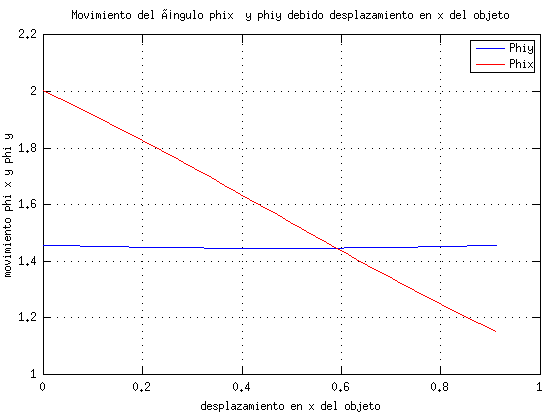
\includegraphics[width=0.6\textwidth]{./pictures/figure1}
   	\caption{}\label{fig: figura}
   \end{figure}
    En la gráfica de la figura 3.1 se puede observar la variación de los ángulos $\phi_x$ y $\phi_y$ con la persona en una única posición: $P=[0, -(L_y+L-H_y), 1]^T$, la variación de la figura en pantalla (en el eje $x$ y $y$) de lo que observan es graficada con el marco de referencia centrado en la esquina superior izquierda de la pantalla, sin embargo los cálculos se hacen tomando la posición de la cámara como marco de referencia. El mayor cambio que ocurre en los ángulos es con respecto a $\phi_x$ de 2 a 1.1 radianes que son 0.9 radianes o 51.5662 grados, lo cual parece tener mucho sentido ya que el desplazamiento se hace en el eje de $\phi_x$. 
    \\Lo que resulta peculiar es que a pesar de que no hay desplazamiento en el eje y de la figura  si hay una ligera variación en el ángulo $\phi_y$ de la mirada de la persona, esto se debe al punto de fuga. El punto de fuga es el lugar geométrico en el cual las proyecciones de las rectas paralelas a una dirección dada en el espacio, no paralelas al plano de proyección, convergen, lo anterior se puede ver ilustrado en la figura 3.2, el punto de fuga es el lugar donde convergen todas líneas "paralelas" de color verde, y la línea del horizonte es la recta horizontal de color azul.
    \begin{figure}[htbp]
    	\centering
    	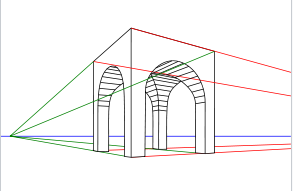
\includegraphics[width=0.3\textwidth]{./pictures/fuga}
    	\caption{}\label{fig: figura}
    \end{figure}
    Cuando la figura inicialmente se encuentra en una posición superior a la de los ojos y se mueve hacia uno de los extremos de la pantalla, ésta pareciera moverse hacia abajo (hacia el horizonte) y cuando inicialmente la figura se encuentra en una posición inferior a la de los ojos de la persona y se mueve hacia un extremo, ésta pareciera moverse hacia arriba por lo tanto la mirada de las personas en el eje $y$ tiende a moverse.
    
    \begin{figure}[htbp]
    	\centering
    	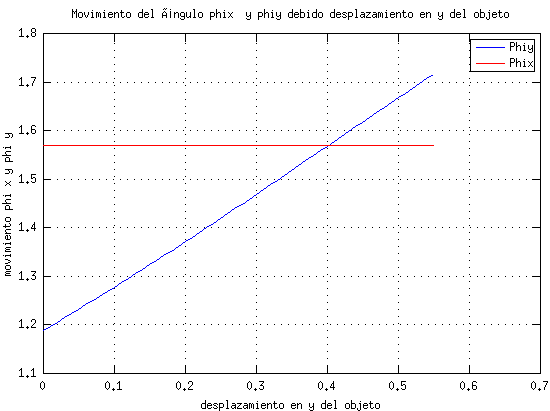
\includegraphics[width=0.6\textwidth]{./pictures/figure2}
    	\caption{}\label{fig: figura}
    \end{figure}
    En la gráfica de la figura 3.3	se puede apreciar que el objeto que observan las personas en pantalla únicamente se desplaza en el eje $y$, en este caso el único desplazamiento de la mirada es con respecto al ángulo  $\phi_y$, al desplazarse el objeto de $0.5523m$ la mirada varía de $1.2$ a $1.7$ radianes, es decir, $0.5$ radianes o lo que e lo mismo $28.6479$ grados.
     \begin{figure}[htbp]
     	\centering
     	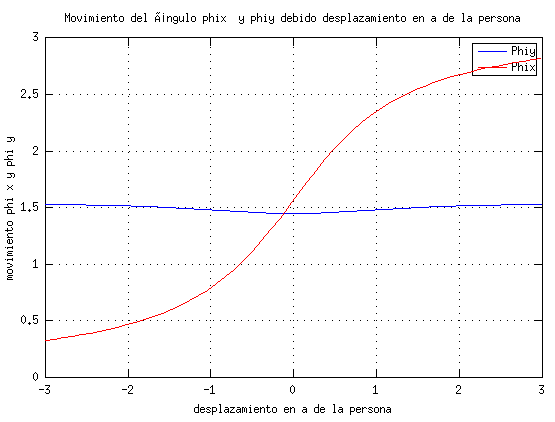
\includegraphics[width=0.6\textwidth]{./pictures/figure3}
     	\caption{}\label{fig: figura}
     \end{figure}
     
     La gráfica 3.4 describe el caso en el únicamente la  persona se mueve sobre el eje $X$ de $-3$ a $3$m, el mayor desplazamiento lo tiene el ángulo $\phi_x$, de esta gráfica se puede concluir que la mayor variación en el ángulo se da entre $-1$ y $1m$ la cual la mirada varía de $0.8$ a $2.36$ radianes, si la persona se mueve más allá de esta distancia la mirada tiende a estabilizarse y no valdría la pena hacer experimentos en estas zonas. Lo anterior se ve con mayor claridad en la figura 3.5, aquí se amplio el rango en el que se mueve la persona sobre el eje $X$ y en consecuencia $\phi_x$ tiende a estabilizarse.
     \begin{figure}[htbp]
     	\centering
     	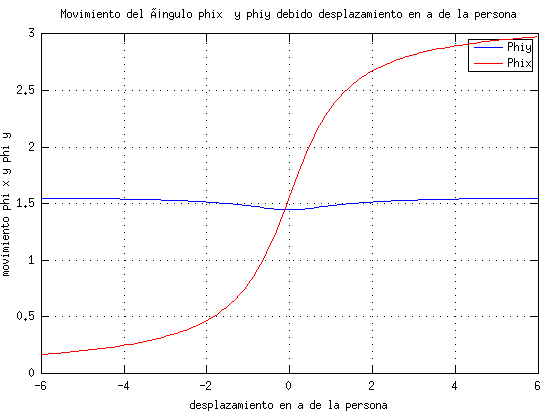
\includegraphics[width=0.6\textwidth]{./pictures/figure5}
     	\caption{}\label{fig: figura}
     \end{figure}
     
     El último análisis corresponde al caso cuando la figura en pantalla no se mueve y la persona únicamente se mueve sobre el eje $Z$. La figura que observa se encuentra en el centro de la pantalla, es decir en: $[S_x, S_y, S_z]^T=[\frac{W}{2}, -(c_y+\frac{L}{2}), 0]^T$ y la persona se encuentra en $[P_x, P_y, P_z]^T=[0, -(L_y+L-H_y), vecZ]^T$ donde $vecZ$ es un vector que va desde $0.1$ a $3m$.
      \begin{figure}[htbp]
      	\centering
      	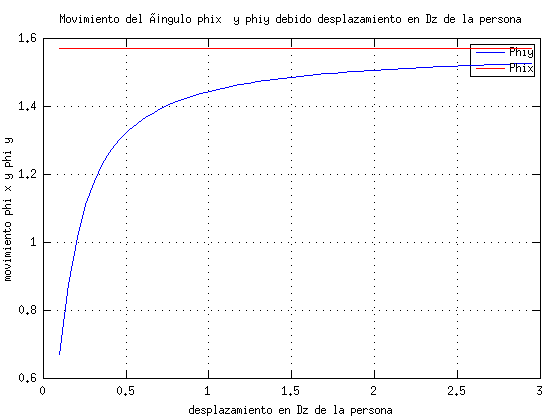
\includegraphics[width=0.6\textwidth]{./pictures/figure4}
      	\caption{}\label{fig: figura}
      \end{figure}
      En la gráfica 3.6 se puede apreciar que mientras se va alejando la persona el único ángulo de la mirada que varía es $\phi_y$, va de $0.6 a 1.55$ radianes, esto quiere decir que hay una variación en el ángulo de 0.95 radianes o 51.56 grados hacia abajo cuando la persona se aleja, además se puede observar que a partir de 1.5m la variación que hay es muy pequeña, de 0 a 0.8m es cuando se da la mayor variación. Lo anterior se puede explicar  con la linea de fuga, mientras la persona se aleja el objeto pareciera moverse hacia abajo y establecer con la mirada de la persona en 1.6 radianes o 91 grados, en el horizonte.

      \subsection{Desviación de $\phi_y$ y $\phi_x$. Segundo caso}
      El segundo caso para calcular $\phi_y$ y $\phi_x$ es un tanto similar al primero pero con la diferencia de que para obtener dichos ángulos no es necesario que la cámara (origen) se encuentre en una rotación específica (paralela al piso) como en el caso anterior. Ahora los ángulos se calculan de manera independiente a la orientación de la camára, para lograr lo anterior únicamente se necesita conocer cual es la ecuación del piso con respecto a la cámara, la ubicación de la persona en el plano y su estatura. En las secciones siguientes se explica como se obtienen los parámetros del plano del piso $n$ (normal del plano) y $d$ (distancia más cercana al origen) mediante técnicas de visión computacional y geometría proyectiva.\\

      %Poner un poco de info de cosenos directores en el marco
      \subsubsection{Localización de P}
	    Como se mencionó anteriormente para hallar la mirada de las personas en los dos ángulos únicamente se necesita aplicar la fórmula de cosenos directores al punto $P$ (cabeza de la persona) y $S$ (objeto en pantalla).
      Sea $F=[F_x, F_y, F_z]$ un punto que yace en el piso donde se coloca la persona. $F$ se puede obtener estableciendo dos valores en la ecuación del plano, uno en el eje $x$ y el otro en el eje $z$ y el valor de $y$ se consigue despejando el la variable $y$ de la ecuación:
        \begin{eqnarray}
        y=\frac{d-Ax-Cz}{B}
        \end{eqnarray}
      De la ecuación anterior $F_x=x$, $F_y=y$ y $Fz=z$. Para encontrar $P$ simplemente se parte de $F$ y multiplicamos la estatura de la persona $H_y$ en dirección negativa (regla de la mano derecha) por la norma de la normal del plano, lo anterior se debe a que las personas al estar paradas sobre el piso siempre están paradas de una manera ortogonal, el resultado de esta operación es la ubicación de $P$ en 3 dimensiones.\\
      %Tal vez hablar de la regla de la mano derecha
      \begin{figure}[htbp]
       	\centering
       	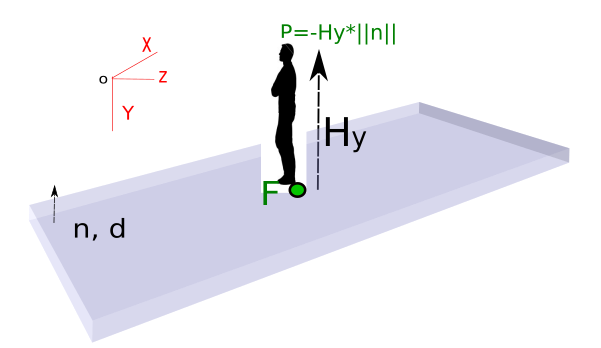
\includegraphics[width=0.5\textwidth]{./pictures/calculoP}
       	\caption{}\label{fig: figura}
      \end{figure}

       \subsubsection{Localización de S}
       Para conocer con precisión cual es la ubicación en pantalla del objeto con respecto a la cámara como marco de referencia con la cámara en cualquier orientación se hizo uso de una unidad Pan-Tilt. Una unidad Pan-Tilt es un dispositivo que permite colocar camáras  en posiciones muy precisas, imagen \ref{pantilt}.\\
          \begin{figure}[htbp]
           	\centering
           	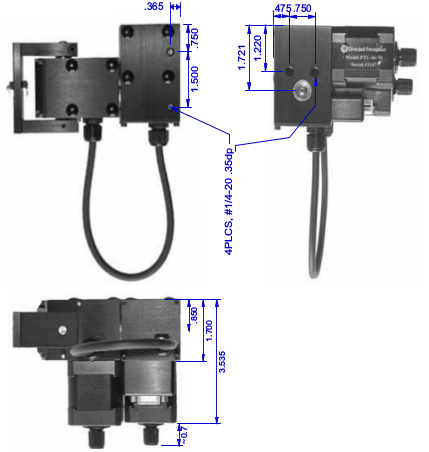
\includegraphics[width=0.2\textwidth]{./pictures/pantilt}
           	\caption{}\label{fig: figura}
           	\label{pantilt}
        \end{figure}
     Sea $O_c$ el eje de rotación de la cámara (punto focal), $O_u$ el eje de rotación de la unidad Pan-Tilt, $D_{cu}$ la distancia en el eje $y$ entre $O_c$ y $O_u$, $\theta$ el ángulo que rota la unidad Pan-Tilt alrededor del eje $X$, $S_1=(S_{1x}, S_{1y}, S_{1z})$ la ubicación inicial de la figura en pantalla antes de la rotación de la unidad y $S_2$ la ubicación después de la rotación, figura \ref{pantilt2} y \ref{pantilt3}. Conociendo $S_1$ con respecto al marco de referencia de la cámara la localización de $S_2$ se realiza tomando en cuenta los parámetros anteriores mediante los siguientes pasos:
              \begin{figure}[htbp]
              	\centering
              	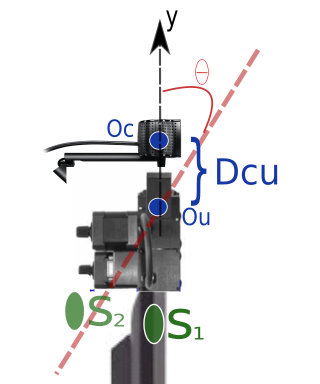
\includegraphics[width=0.3\textwidth]{./pictures/pantilt3}
              	\caption{}\label{fig: figura}
              	\label{pantilt3}
              \end{figure}
      \begin{itemize}
      	\item Colocando la unidad Pan-Tilt con la cámara de manera que el objetivo de la cámara quede de forma perpendicular a la al plano de la pantalla en la cual se proyectarán las figuras que los sujetos de experimentación observarán, lo anterior observando desde el plano $Y-Z$ del marco de referencia.
       \begin{figure}[htbp]
       	\centering
       	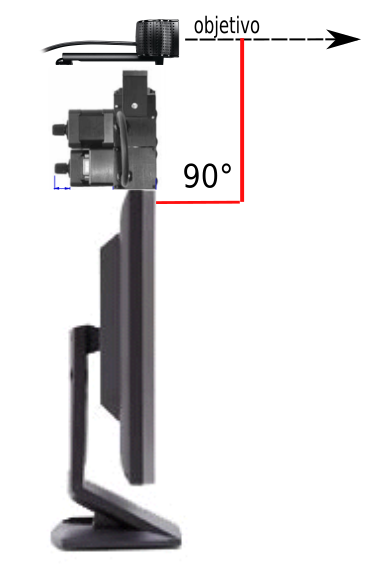
\includegraphics[width=0.2\textwidth]{./pictures/pantilt2}
       	\caption{}\label{fig: figura}
       	\label{pantilt2}
       \end{figure}
      	
      	\item Se traslada el punto $S_1$ hacia el eje de rotación de la cámara $O_c$ mediante $D_{cu}$ metros, únicamente desplazándolo en el eje $Y$.
      	\item Se rota $\theta$ grados el punto a través de la matriz de rotación del eje $X$.
      	\item Finalmente se regresa el punto $D_{cu}$ metros.
      \end{itemize}
	Lo anterior se realiza con la siguiente ecuación:
	%\tiny{		
	        \begin{eqnarray}
	        S_2=
	        \begin{bmatrix}
	        1 & 0 & 0\\
	        0 & cos(-\theta) & -sen(-\theta)\\
	        0 & sen(-\theta) & cos(-\theta)
	        \end{bmatrix}*\begin{bmatrix}S_{1x}\\
	         S_{1y}-D_{cu}\\
	          S_{1z}
	        \end{bmatrix}+\begin{bmatrix}S_{1x}\\
	        S_{1y}+D_{cu}\\
	        S_{1z}
	        \end{bmatrix}
	        \end{eqnarray}
     % }
      
      \section{Simulación processing}
      Se realizó una simulación mediante el software processing del análisis anterior, esto se hizo para poder observar el comportamiento de los ángulos en diferentes posiciones de las personas al mismo tiempo y variar en tiempo real y de manera interactiva la posición en el eje $X$ y $Y$ de la figura en pantalla. Los parámetros del escenario son los mismos a los utilizados en la análisis anterior: $W$, $L$, $LY$, $Cy$ y $Hy$. \\
      En la figura 4.1 se puede apreciar una figura de la simulación, en ella se despliegan 36 posiciones de personas separadas por 1m en el eje $X$ y 0.5m en el eje $Y$. La variación en el eje $Y$ se da por medio de la barra deslizante que se encuentra en la esquina inferior derecha, va de 0 a 0.5523m y el desplazamiento en el $Y$ se logra haciendo click en la figura (óvalo blanco) en pantalla que se encuentra en la parte superior de la ventana de la simulación y sin soltar el mouse se arrastra la figura de izquierda a derecha. Los ángulos $\phi_x$ y $\phi_y$ además de ser mostrados en cada una de las posiciones son representados mediante el radio del círculo que representa cada persona y la línea que sale de dicho ángulo, $\phi_x$ es la línea y $\phi_y$ es el radio.\\
      \begin{figure}[htbp]
      	\centering
      	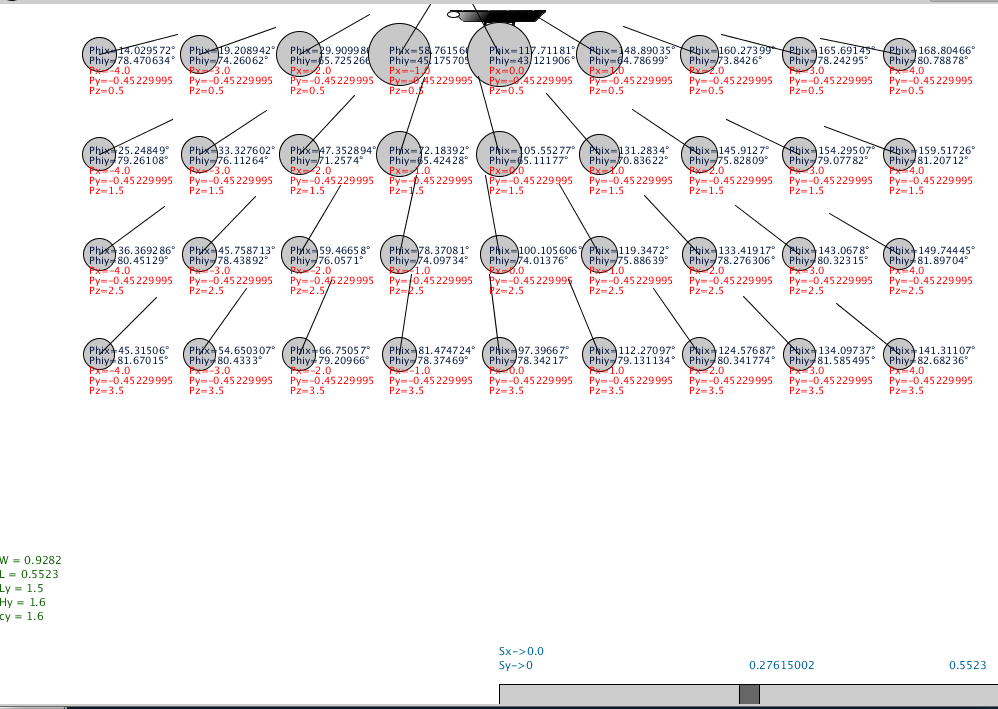
\includegraphics[width=1\textwidth]{./pictures/sim}
      	\caption{}\label{fig: figura}
      \end{figure}
      Mediante la simulación de igual manera se demostró como al arrastrar la figura únicamente en $X$ no solo varía $\phi_x$ sino también $\phi_y$ de todas las instancias, esto se puede corroborar en los valores de los ángulos y en el área del círculo.
      
      %Debo detallar más la programación en esta sección?: Clases, funciones
        \section{Dispositivo para adquirir datos}
        Durante la etapa de adquisición de datos para el algoritmo de entrenamiento, además de conocer la ubicación de la persona y la de la figura que observan en pantalla es necesario capturar una imagen del rostro de la persona y conocer (mediante un aparato de medición) la orientación de la cabeza, lo anterior es necesario para evaluar y compararar el sistema de estimación de pose. \\
        Como señalan en [Murphy-Chutorian, 2009] el método que se utilice para obtener las medidas de la orientación de la cabeza en el conjunto de entrenamiento debe ser preciso y entre los métodos más eficientes proponen los sistemas captura ópticos de movimiento y los sensores inerciales, sin embargo, los primeros son muy costosos, por lo que en el desarrollo del presente trabajo de tesis se optó por utilizar un sensor inercial, el cual consiste de acelerómetros y giroscopios a menudo acoplados con algún tipo de filtro para reducir ruido.
        
        En este apartado se describirá el proceso de diseño y fabricación del dispositivo que realiza la medición de la orientación.\\
        De modo que la tarjeta electrónica debe ir en la cabeza de las personas, durante el diseño se tomó mucho en cuenta el tamaño y el peso que tendría, ya que de ser muy grande y  pesado podría ser muy incomodo para las personas durante los experimentos. 
        \subsection{IMU}
        El imu seleccionado para este proyecto es el BNO055 de Bosch (figura 5.1). El sensor utiliza algoritmos que mezclan los datos del acelerómetro, magnetómetro y giroscopio en una salida estable de la orientación de los tres ejes, el sensor es capaz de arrojar los datos en cuaterniones, vectores y ángulos de Euler. El BNO055 se alimenta con voltaje de 3.3 a 5v, mide 2.67x2.032cm y para obtener los datos utiliza comunicación I2C.
        
        \begin{figure}[htbp]
        	\centering
        	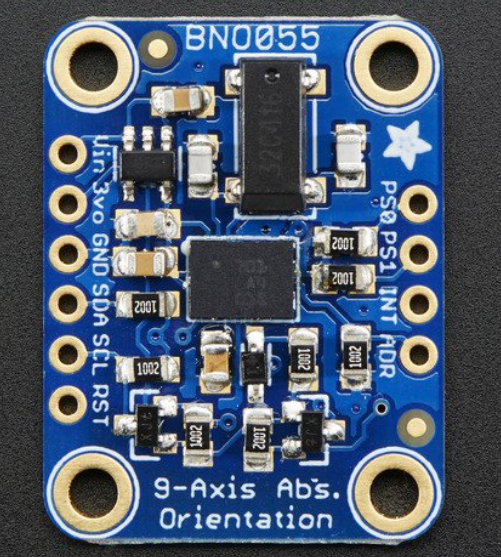
\includegraphics[width=0.5\textwidth]{./pictures/bno055}
        	\caption{}\label{fig: figura}
        \end{figure}
        
        \subsection{Microcontrolador}
        Debido a las restricciones de peso y tamaño se utilizó un arduino micro, el cual es la versión más pequeña del arduino con 4.8x1.8cm y esto se debe a que es una versión más limitada en cuanto a periféricos y módulos, sin embargo, es adecuada para el uso que se le da en el proyecto, únicamente se utilizará para obtener los datos del imu mediante comunicación I2C y enviarlos a la computadora por comunicación serial. El arduino se alimenta mínimo con 7v para que su regulador interno regule a 5v el microcontrolador que usa.
        \begin{figure}[htbp]
        	\centering
        	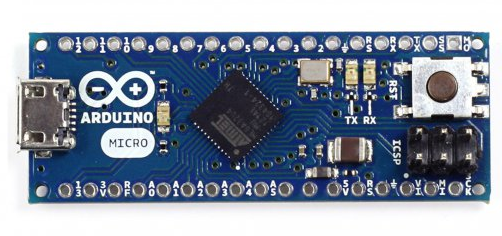
\includegraphics[width=0.5\textwidth]{./pictures/arduino}
        	\caption{}\label{fig: figura}
        \end{figure}
        
        \subsection{Xbee}
        Durante los experimentos las personas se estarán moviendo en diferentes posiciones de la escena y mirando diferentes lugares en la pantalla, como se había mencionado la tarjeta electronica se colocará en su cabeza, por lo que utilizar un cable (de comunicación serial) entre la computadora y la tarjeta para obtener los datos de la pose sería muy inadecuado ya que éste debe ser bastante largo, le pesaría a la tarjeta y afectaría su posición en la cabeza, y finalmente podría afectar la experiencia de la persona el tener un cable muy extenso cerca de ella. Tomando en cuenta las consideraciones anterior se decidión trabajar con módulos xbee.\\
        Los xbee son módulos inalámbricos creados para la comunicación inalámbrica entre ellos, su finalidad es la eliminación de cables en la comunicación serial. Para este proyecto se utilizaron los xbee s1 (figura 5.3) los cuales son los más  pequeños, de bajo consumo y simples de utilizar debido a que su configuración punto a punto es bastante sencilla y únicamente se requiere declarar un xbee como emisor y el otro como receptor. Los xbee s1 se alimentan con 3.3v.
        
        \begin{figure}[htbp]
        	\centering
        	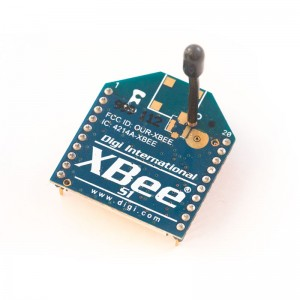
\includegraphics[width=0.4\textwidth]{./pictures/xbee}
        	\caption{}\label{fig: figura}
        \end{figure}
        
        \subsection{Diseño de la tarjeta}
        Para alimentar todo el circuito es necesario al menos 7v, ya que como se habíía mencionado eso necesita el Arduino micro y es el dispositivo que requiere mayor voltaje, el imu funciona con 5v por lo que se le puede conectar el pin de 5v que tiene el Arduino, sin embargo aún se tiene el inconveniente de que el xbee y su comunicación funcionan con 3.3v, y las baterías recargabales de iones de litio como la que se pretende utilizar por su reducido tamaño y peso, arrojan solo 3.7.v.\\
        Para solucionar el problema de los 7v se utilizó la bomba de carga TPS61093, figura 5.4, en una configuración para elevar el voltaje a 7v. La comunicación entre el arduino y el xbee (diferentes niveles de voltaje) se logró mediante el cambiador de nivel TXS0102, y finalmente para obtener 3.3v de la batería se utilizó el regulador TPS73633. Se pudo alimentar el xbee a través del pin de 3.3v del arduino, sin embargo, el xbee consume hasta 60mA lo cual es demasiado para el regulador de 3.3v del Arduino y podría afectar su funcionamiento.
        
        \begin{figure}[htbp]
        	\centering
        	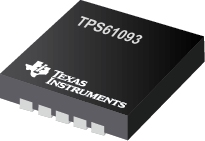
\includegraphics[width=0.2\textwidth]{./pictures/TPS61093}
        	\caption{}\label{fig: figura}
        \end{figure}
        En la imagen 5.5 se puede ver el esquemático de la tarjeta y en la 5.6 el pcb.
        \begin{figure}[htbp]
        	\centering
        	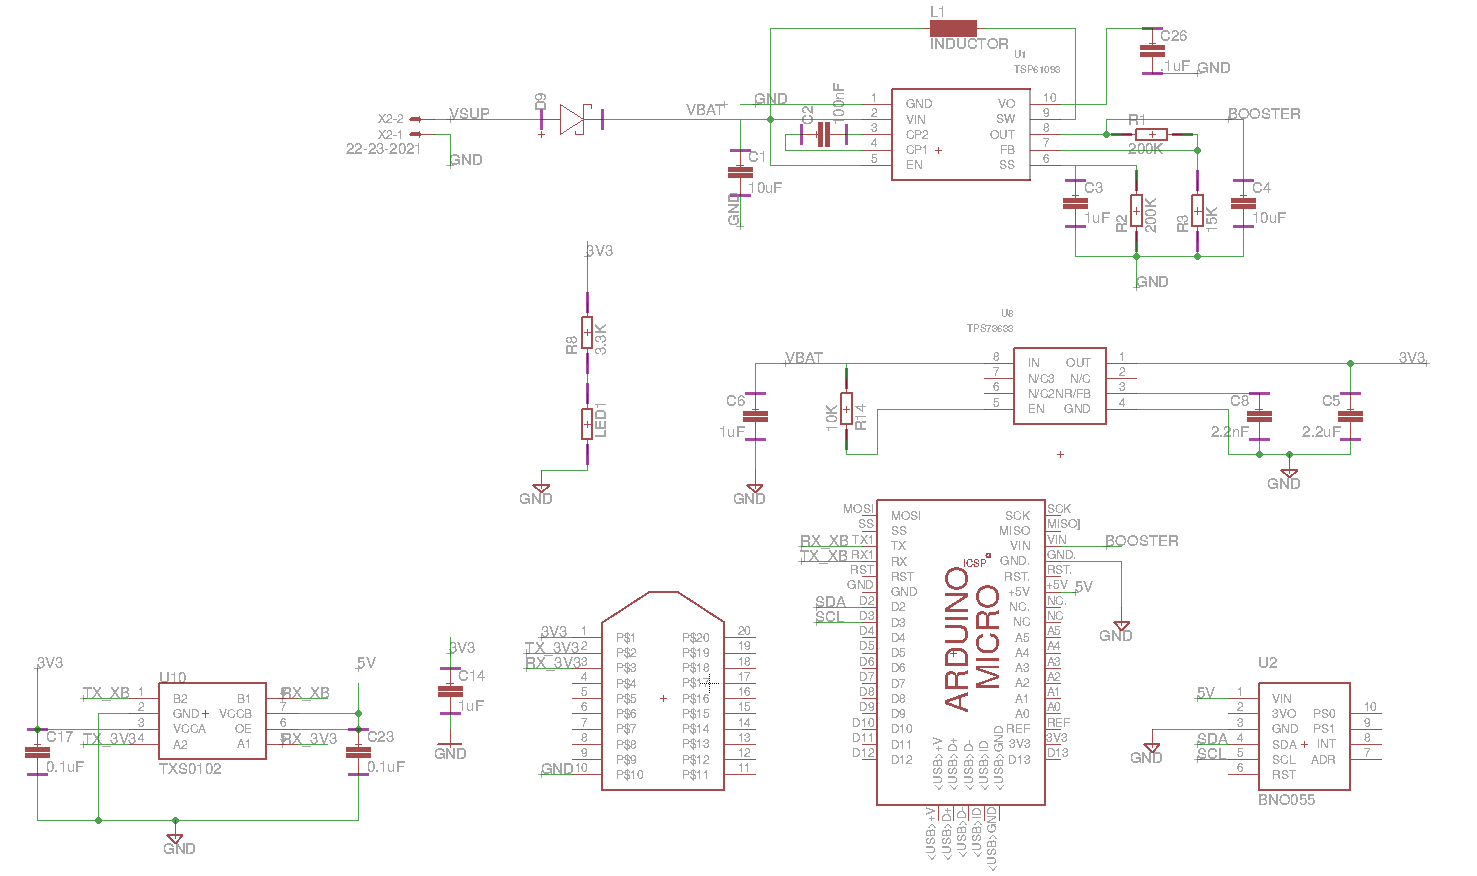
\includegraphics[width=1.\textwidth]{./pictures/schematic}
        	\caption{}\label{fig: figura}
        \end{figure}
        \begin{figure}[htbp]
        	\centering
        	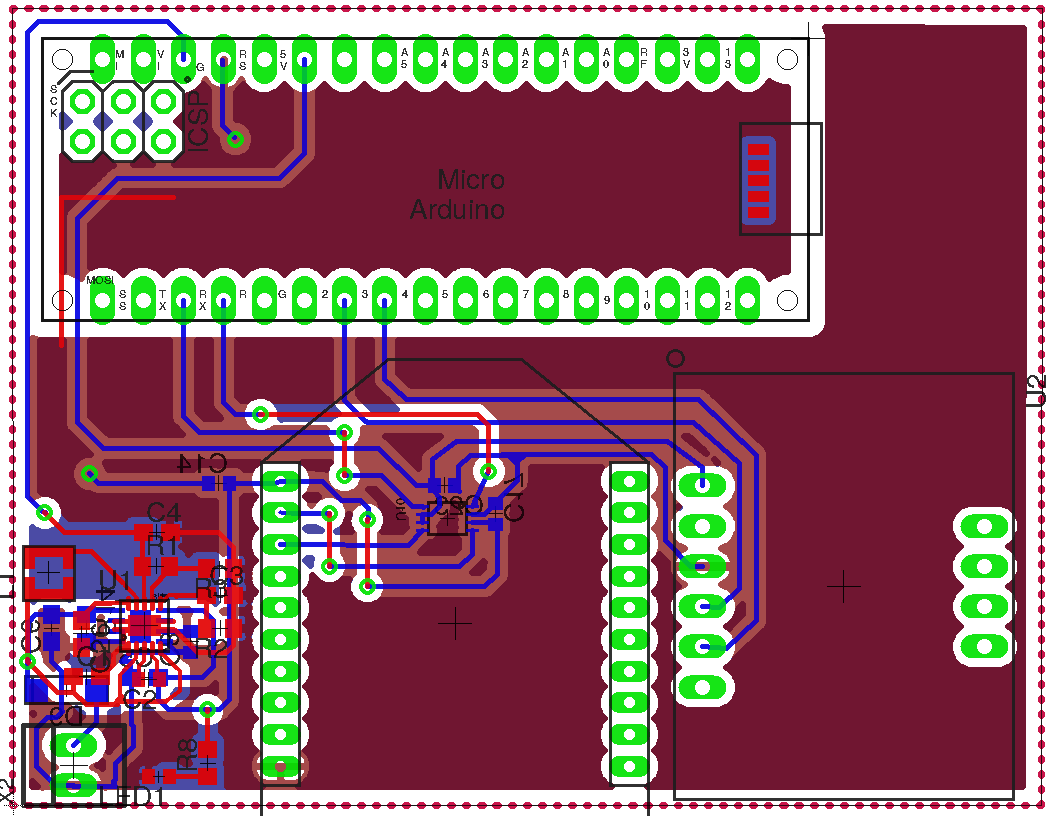
\includegraphics[width=1.\textwidth]{./pictures/board}
        	\caption{}\label{fig: figura}
        \end{figure}
        Adicionalmente se creo una pequeña tarjeta para la recepción de datos a través del otro xbee y envío a la computadora mediante un cable con convertidor de rs232 a usb. Más adelante se detallará el programa para la recepción de datos.
        
        \subsection{tarjeta electrónica}
        En las siguientes imágenes se presentan: la tarjeta electrónica con el imu, arduino y xbee ya fabricada; la batería recargable de 3.7v y la tarjeta que conecta el xbee receptor de datos con la computadora para poder enviar los datos del imu hacia la computadora.
        \begin{figure}[htbp]
        	\centering
        	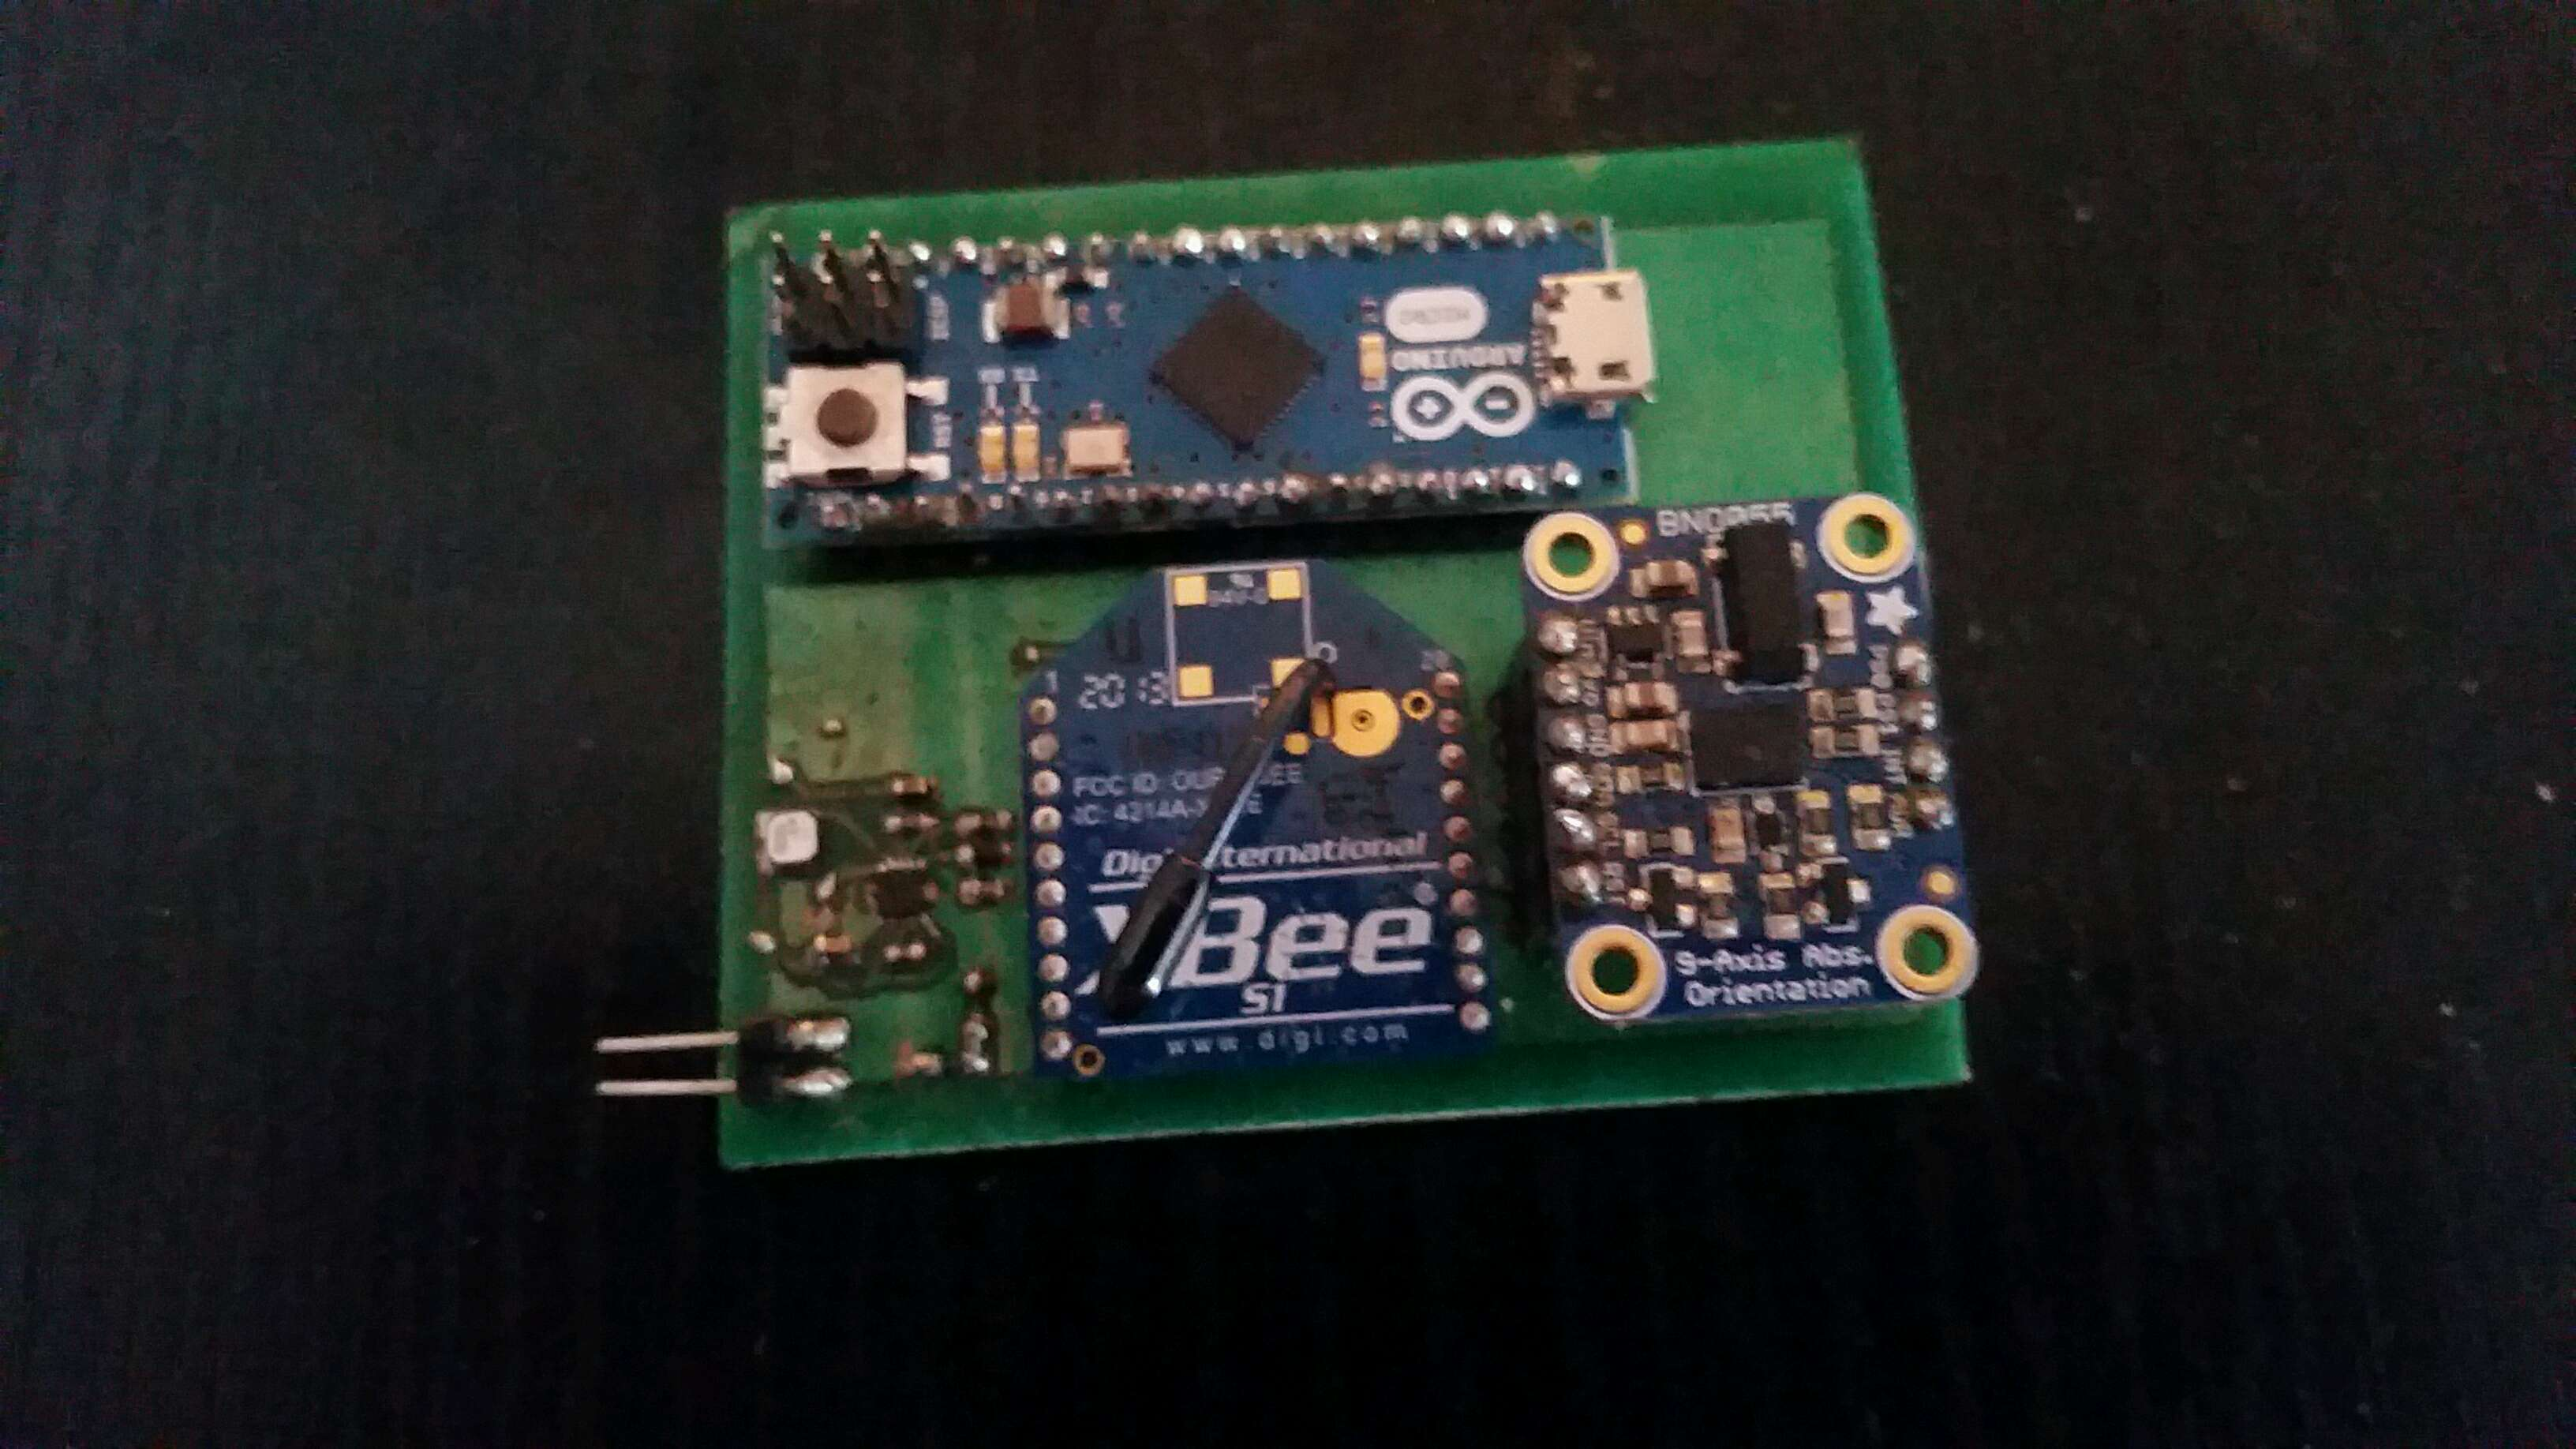
\includegraphics[width=.5\textwidth]{./pictures/placa1}
        	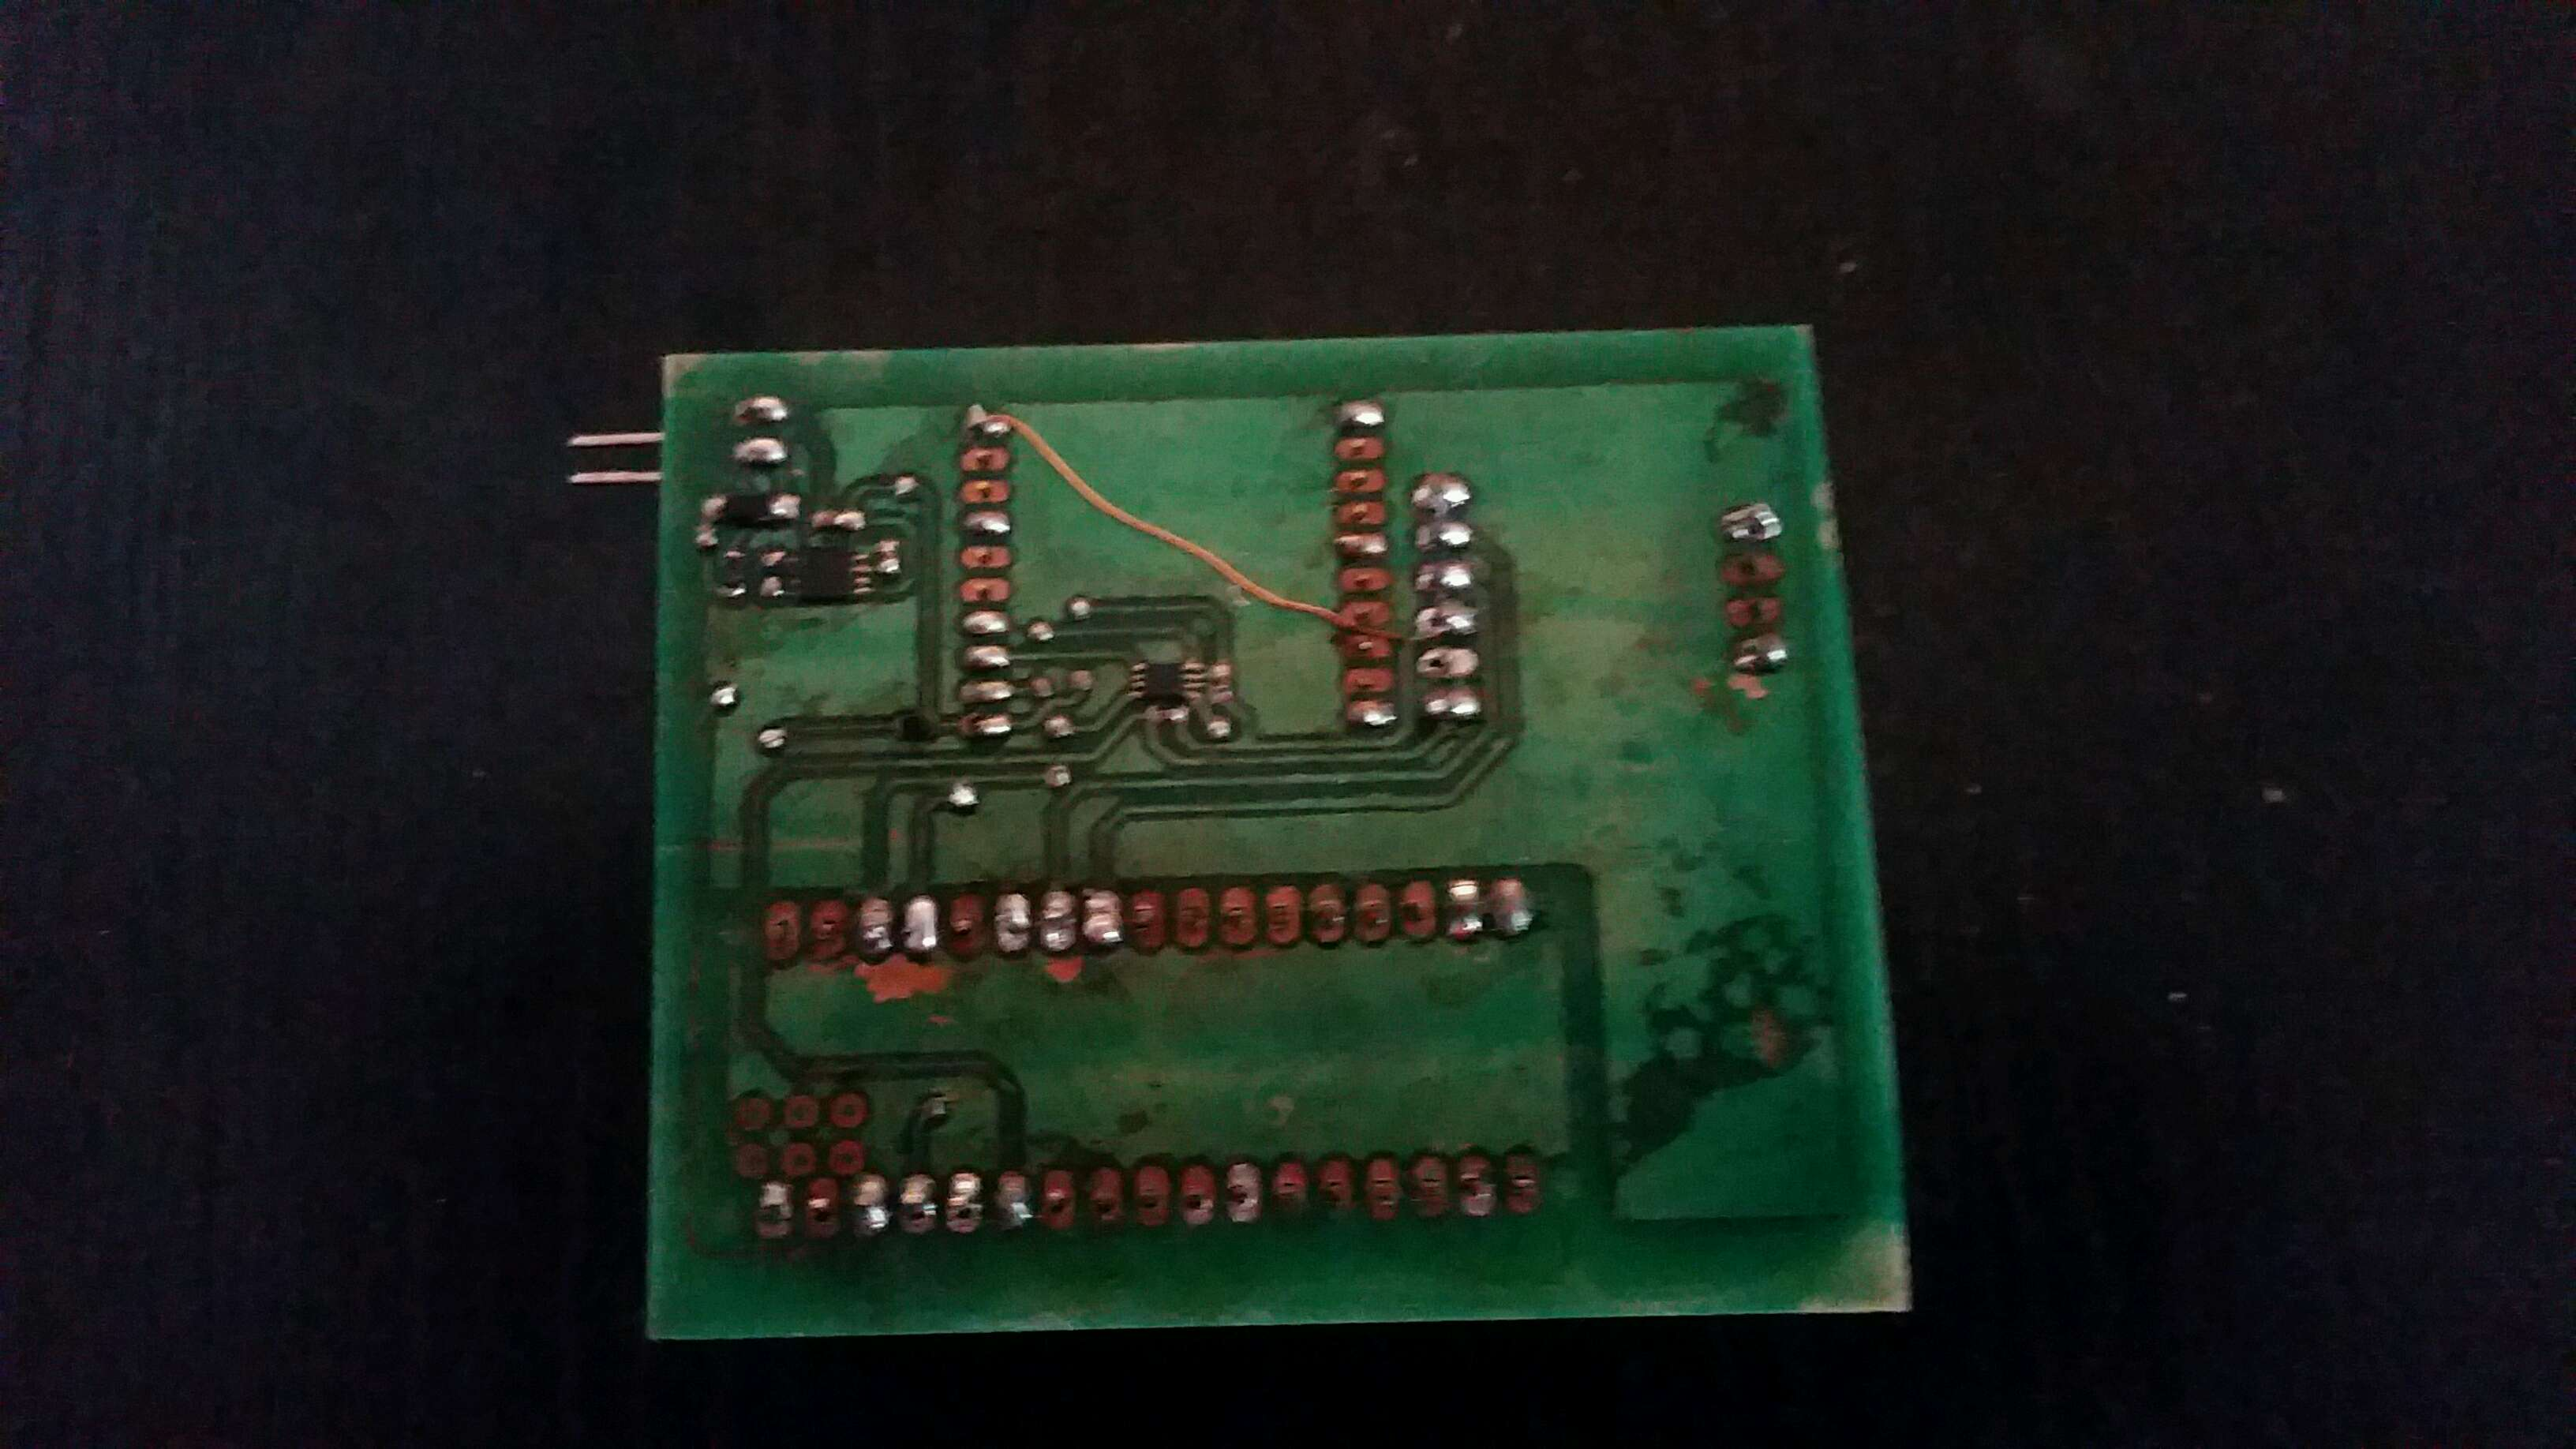
\includegraphics[width=.5\textwidth]{./pictures/placa2}
        	\caption{tarjeta con el IMU}\label{fig: figura}
        \end{figure}
        \begin{figure}[htbp]
        	\centering
        	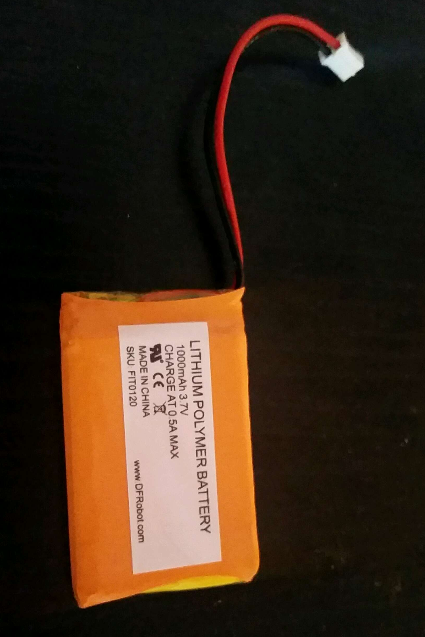
\includegraphics[width=.3\textwidth]{./pictures/pila}
        	\caption{batería recargable}\label{fig: figura}
        \end{figure}
        
        \begin{figure}[htbp]
        	\centering
        	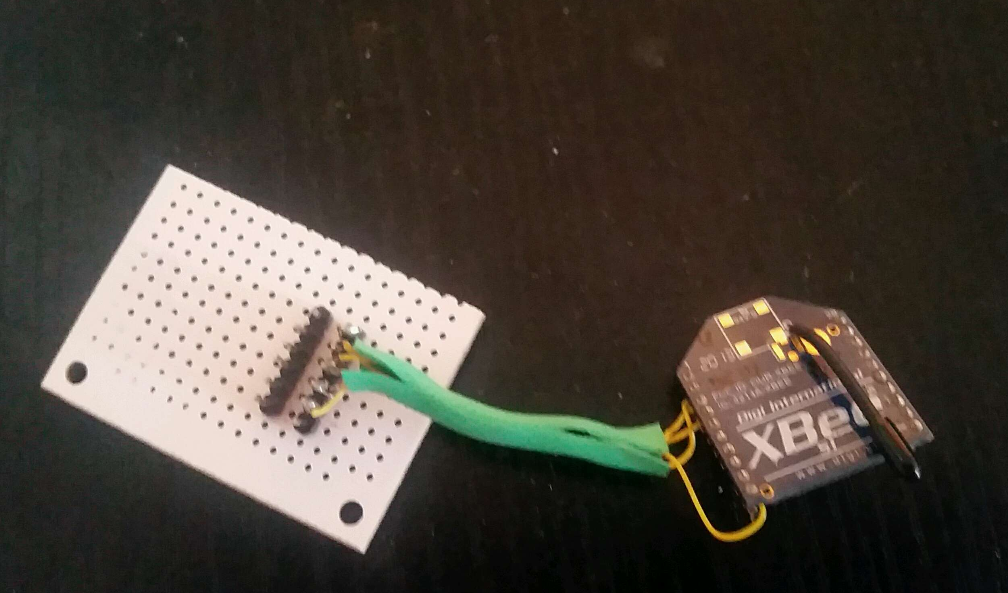
\includegraphics[width=.5\textwidth]{./pictures/placa3}
        	\caption{tarjeta receptora de datos}\label{fig: figura}
        \end{figure}
        
       \section{Rotaciones en los pares de posiciones}
       Se eligió como forma de representación de la pose de la cabeza los cuaterniones, los cuales son obtenidos mediante el IMU, como se había mencionado el dispositivo se colocará en la cabeza de las personas durante el entrenamiento para la generación del "ground truth", sin embargo, aún falta considerar los siguientes detalles:
       \begin{itemize}
       	\item ¿Cuáles posiciones en el piso con respecto al marco de referencia centrado en la cámara  se utilizaron para capturar la información(imagen rostro y pose en cuaterniones)?.
       	\item ¿A quá distancia estarán las posiciones entre si y hasta que distancia máxima se tomarán datos, es decir, cual es el mínimo en $X$ y $Z$ que se debe seleccionar? ya que como se observó en la sección de \textit{Análisis del comportamiento de los ángulos $\phi_x$ y $\phi_y$} dependiendo de los parámetros del experimento hay valores en los cuales ya no vale la pena hacer análisis ya que las variaciones en los ángulos es muy pequeño o inexistente.
       	\item ¿Cuáles posiciones para la figura en pantalla se deben utilizar?.
       	\item ¿Cuántas posiciones de figura en pantalla y personas en el piso se considerarán?
       	\item ¿Cómo lidiar con las pequeñas variaciones en las mediciones del IMU que se den en diferentes personas en los mismas instancias de experimentación?
       	
       \end{itemize} 
       
       \subsection{Cálculo de todas las rotaciones posibles}
          \section{Proyección de marcas en el piso}
          Como se mencionó anteriormente para la etapa de entrenamiento del algoritmo de apendizaje automático se debe tener control sobre las capturas que se van a tomar de cada sujeto de experimento incluyendo las posiciones en la escena donde se colocarán al capturar los datos.
          Una vez calculada las mejores posiciones en la escena para capturar los datos con las que se va a entrenar el algoritmo, la siguiente etapa consiste en colocar estos puntos con marcas en el piso para saber durante los experimento en qué posiciones se deben colocar las personas.
          Como se había mencionado las marcas son con respecto al marco de referencia centrado en la cámara, la cual se encuentra sobre la pantalla, dichas marcas se pueden pintar en el piso midiendo sus coordenadas a partir de la cámara mediante un flexómetro o cinta métrica, sin embargo al realizarlo de esta forma se tienen los siguientes problemas:
          \begin{itemize}
          	\item Hay bastante inexactitud, por ejemplo en caso de que no se mida sobre la misma dirección de los ejes debido a pequeños \underline{errores humanos} y esto tiende a agravarse cuando las marcas son lejanas.
          	\item El sistema de coordenadas centrado en la cámara no es paralela al plano del piso donde se colocarán las marcas ya que se debe rotar en dirección al piso para así tener una mejor vista de los rostros de las personas que se encuentran más cercanas a la cámara. Por lo tanto si rotamos la cámara de igual manera rotamos el marco de referencia y es más complicado colocar las marcas, lo anterior se puede ver ilustrado en la figura 11.1. 
          \end{itemize}
          \begin{figure}[htbp]
          	\centering
          	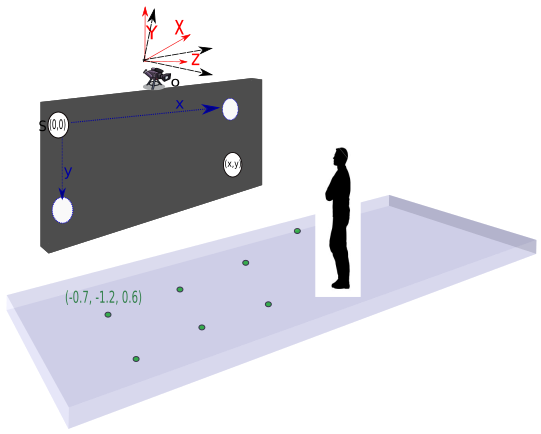
\includegraphics[width=.6\textwidth]{./pictures/ejesRot2}
          	\caption{}\label{fig: figura}
          \end{figure}
          Como solución al problema anterior se desarrollaron algoritmos utilizando visión computacional, geometría y optimización numérica para colocar en el piso de manera más precisa las marcas, el método consiste en conocer cual es la distancia y orientación del plano del piso donde se situarán las personas y  proyectar las marcas en éste tomando como marco de referencia la cámara.
              \subsection{Proyección de marcas mediante visión computacional, geometría y optimización numérica}
              %Se puede explicar a grandes rasgos en que consiste homografía, R y T proyección en el piso y luego detallar
              Para utilizar el método que se describirá a continuación es necesario conocer la matriz de parámetros intrínsecos $K$. La obtención de esta matriz se logró mediante el software de Matlab: Camera Calibration Toolbox, dando como resultado la siguiente matriz.
              \[K=
              \begin{bmatrix}
              fx & 0 & c_x\\
              0 & f_y & c_y\\
              0 & 0 & 1
              \end{bmatrix}
              =
              \begin{bmatrix}
              616.164 & 0 & 325.528\\
              0 & 616.82 & 228.66\\
              0 & 0 & 1
              \end{bmatrix}
              \]
       \subsubsection{Homografía}
       Durante la primera etapa se debe hallar la homografía que mapea puntos en el plano del piso y los respectivos puntos en la imagen de ese plano, todas coordenadas deben estar en metros, los puntos en el plano del piso deben tener las medidas reales que hay entre ellos, tener uno de los puntos como origen y con respecto a éste establecer las coordenadas de las demás.\\
       La matriz de homografía se descompone y a partir de ella se encuentra la matriz de rotación y el vector de traslación que existe entre el plano del piso y la cámara, es decir, este método se basa en un modelo conocido 3D y su correspondencia en el plano imagen 2D.\\
       Inicialmente se creó un software para capturar con el mouse 4 puntos marcados en el piso siguiendo un orden en específico, la matriz con los puntos establecidos con las medidas reales se denomina $scnPts_{4x4}$ y la matriz obtenida con los puntos capturados con el mouse se denomina $imgPts_{3x4}$. Los puntos establecidos en el piso tienen forma cuadrangular y están separados entre sí a $0.4m$, tomando como origen el punto de la esquina superior izquierda y como primera captura, como segundo punto la esquina inferior izquierda, tercer punto la esquina inferior derecha y último la esquina superior derecha establecemos la siguiente matriz:
       \[scnPts=
       \begin{bmatrix}
       0 & 0 & 0.4\\
       0 & 0.4 & 0.4\\
       0 & 0 & 0\\
       1 & 1 & 1 
       \end{bmatrix}
       \]
       donde cada columna es un punto, la primera fila representa la coordena en el eje $x$, la segunda en $y$ y la tercera en $z$. Nótese que son coordenadas homogéneas y el valor en $z$ es cero ya que todos los puntos yacen sobre el mismo plano. Como se puede observar la matriz $scnPts$ está en metros por lo tanto se requiere que $imgPts$ igual esté en metros, esto se consigue simplemente multiplicando la matriz $imgPts$ por la inversa de la matriz $K$.\\
       Como resultado del proceso anterior se obtuvo una homografía inexacta ya que al comprobar si mapeaba los puntos de la escena a la imagen ésta no lo hacía correctamente, los puntos tenían bastante error.
       El error en la matriz de homografía podría deberse a los siguientes motivos:
       \begin{itemize}
       	\item  Hay una distancia considerable entre los puntos del plano y la imagen
       	\item La captura de los puntos en la imagen mediante el mouse es realizada por simple inspección y seleccionando los puntos lo cual podría generar capturas erróneas.
       	\item Son pocos puntos para calcular la homografía
       \end{itemize}
       Para solucionar los inconvenientes anteriores se optó por utilizar más puntos, para ello se colocó una manta con un tablero de ajedrez con 48 intersecciones o en este caso 48 puntos con una longitud de $12cm$ cada lado, esto quiere decir que los puntos estarán separados a $0.12m$, además con el objetivo de que sea más precisa la captura y automática se modificó el programa para localizar las intersecciones automáticamente mediante bibliotecas de openCV y no estar capturando manualmente los puntos. Ahora la matriz $scnPts$ tiene una dimensión de $4x48$ y imgPts $3x48$. En la imagen 11.2 se pueden notar el buen desempeño que tiene algoritmo al encontrar las intersecciones en la manta con el tablero de ajedrez.
       \begin{figure}[htbp]
       	\centering
       	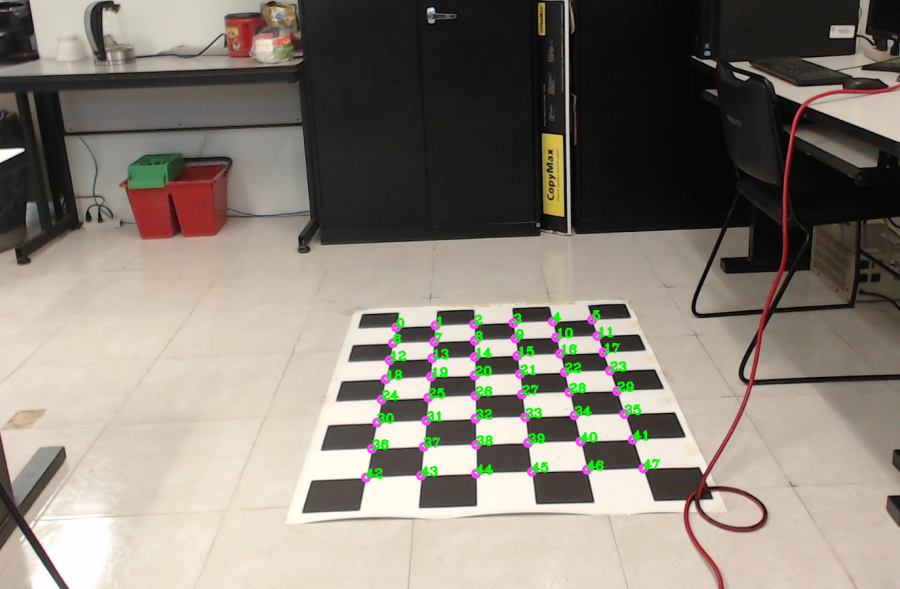
\includegraphics[width=.6\textwidth]{./pictures/ajedrez}
       	\caption{}\label{fig: figura}
       \end{figure}
       
       \subsubsection{Rotación y traslación de la cámara}
       Ya con la homografía $H$ se calcula la pose de la cámara (matriz de rotación $R_{3x3}$ y vector de traslación $T_{3x1}$) con respecto al plano del piso, además, se puede calcular la ecuación del plano la cual será útil más adelante.\\
       \[H=
       \begin{bmatrix}
       h_{11} & h_{12} & h_{13}\\
       h_{21} & h_{22} & h_{23}\\
       h_{31} & h_{32} & h_{3}\\
       \end{bmatrix}
       \]          
       	La primera columna de $H$ contiene la primera columna de $R$ ($R_1$), es decir, la rotación al rededor del primer eje, la segunda columna es la segunda columna de $R$ ($R_2$) y la tercera columna de $H$ es el vector de traslación $T$, solamente queda por calcular la tercera columna de $R$ ($R_3$) la cual tiene que ser ortogonal a las dos primeras, por lo tanto se puede calcular mediante el producto cruz de la primera columna de h con la segunda. Adicionalmente antes de calcular la tercera columna de la matriz de rotación es necesario normalizar $R$ y $T$ debido a redundacias. La normalización se realiza de la siguiente manera:
       	\begin{eqnarray}
       	norm1=||[h_{11} h_{21} h_{31}]^T||\\
       	norm2=||[h_{12} h_{22} h_{32}]^T||\\
       	normT=\frac{norm1+norm2}{2}			
       	\end{eqnarray}
       	\[R=
       	\begin{bmatrix}
       	\frac{h_{11}}{norm1} & \frac{h_{12}}{norm2} & R_{13}\\
       	\frac{h_{21}}{norm1} & \frac{h_{22}}{norm2} & R_{23}\\
       	\frac{h_{31}}{norm1} & \frac{h_{32}}{norm2} & R_{33}\\
       	\end{bmatrix}
       	, T=
       	\begin{bmatrix}
       	\frac{T_x}{normT}\\
       	\frac{T_y}{normT}\\
       	\frac{T_z}{normT}	
       	\end{bmatrix}
       	\]
       	Luego simplemente se aplica el producto cruz para obtener la tercera columna
       	\begin{eqnarray}
       	R_3=R_1 \otimes R_2
       	\end{eqnarray}
       	Para hallar la ecuación del plano con respecto a la cámara (marco de referencia): $Ax+By+Cz=d$ únicamente es necesario la $R$, $T$ de la cámara y un punto de la escena de los que se utilizaron para el cálculo de la homografía.
       	\subsubsection{Cálculo de la ecuación del plano}
       	Como es bien sabido la normal  $n$ al plano $\Pi$ está dado por los componentes: $A$, $B$ y $C$ de la ecuación del plano y la distancia más cercana del plano al origen por: $d$, figura
       	
       	\begin{figure}[htbp]
       		\centering
       		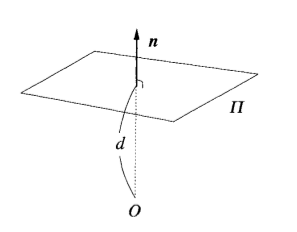
\includegraphics[width=.4\textwidth]{./pictures/plane}
       		\caption{Representación de un plano en el espacio}\label{fig: figura}
       	\end{figure}
       	Tomando como marco de referencia el plano (puntos establecidos en $scnPts$) la normal está dada por el eje $Z$ por lo tanto para obtener la normal con respecto al marco de referencia en la cámara unicamente rotamos este vector con la matriz de rotación:
       	\[n=R*\begin{bmatrix}
       	0\\
       	0\\
       	1	
       	\end{bmatrix}\]
       	Sea $scnPts1_{3x1}$ el primer punto de la matriz de puntos establecidos en la escena, entonces la distancia $d$ del plano al origen es este punto rotado y trasladado hacia la cámara, y al resultado se le aplica el producto punto con la normal al plano:
       	\begin{eqnarray}
       	scnPtsRot=R*scnPts1+T\\
       	d=<N,scnPtsRot>
       	\end{eqnarray}
       	
       	\subsubsection{Reproyección de puntos en la imagen}
       	Todo el proceso anterior fue con el objetivo de poder proyectar puntos en la imagen sobre el plano del piso tomando como marco de referencia la cámara. Lo anterior se consigue únicamente estableciendo la matriz con las marcas en el piso que se necesitan y proyectándolas en la imagen multiplicando por la matriz de parámetros intrínsecos para pasar las coordenadas a pixeles.\\
       	Antes de pasar a esa etapa es necesario verificar que los parámetros encontrados en la sección anterior: $R$, $T$, $n$ y $d$ son correctos. 
       	\begin{itemize}
       		\item La verificación de $n$ y $d$ consiste en utilizar los puntos obtenidos de $imgPts$ y proyectarlos desde el origen hacia el plano (formando rectas) y encontrar las coordenadas en las cuales se intersectan dichas proyecciones con el plano, estas intersecciones deben ser las mismas que las coordenadas de $scnPts$. Sea $L$ la recta en el espacio, $rh$ el vector que va del punto más cercano de $L$ al origen y $m$ el vector unitario que indica la orientación de $L$. 
       		\begin{figure}[htbp]
       			\centering
       			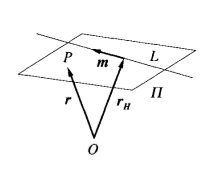
\includegraphics[width=.35\textwidth]{./pictures/intersec}
       			\caption{intersección de una recta con un plano}\label{fig: figura}
       		\end{figure}
       		
       		La intersección de $L$ con el plano $\Pi$ en $r$ está dada por:
       		\begin{eqnarray}
       		r=r_H+\frac{d-<n_{\Pi}, r_H>}{<n_{\Pi},m>}m
       		\end{eqnarray}
       		En este caso las lineas (proyecciones de imgPts) parten de la cámara por lo tanto el vector $rh$ es igual cero, simplificando la ecuación la intersección queda de la siguiente manera:
       		\begin{eqnarray}
       		r=\frac{d}{<n_{\Pi},m>}m
       		\end{eqnarray}	
       		
       		\item La verificación de $R$ y $T$ simplemente se realiza tomando los puntos de $scnPts$ rotándolos, traslandándolos y proyectándolos en la imagen, en caso de que los cálculos de la $R$ y $T$ sean correctos estas proyecciones deben ser las mismas que $imgPts$.
       	\end{itemize}
       	El resultado de los dos comprobaciones se pude ver en la imagen 11.5, las marcas rojas son la proyección en la imagen de la intersecciones con el plano y las verdes son los puntos de $scnPts$ rotados, trasladados y proyectados. Como se puede observar el cálculo de la $n$ y $d$ del plano es bastante precisa, mientras que la $R$ y $T$ tienen error, y parece ser mayor con el desplazamiento sobre el eje $Y$. 
       	\begin{figure}[htbp]
       		\centering
       		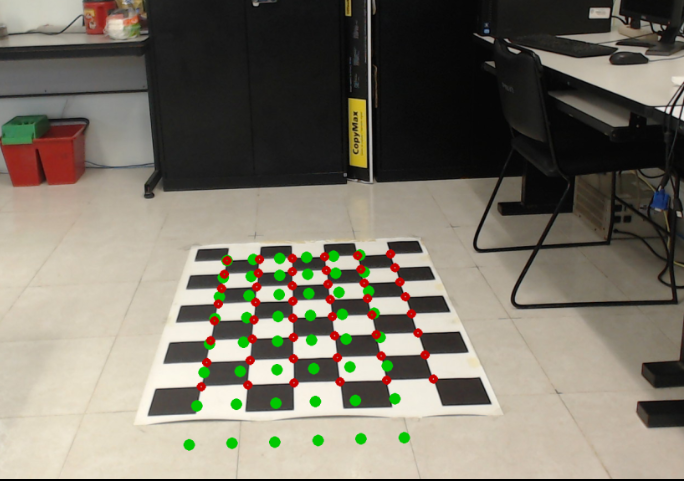
\includegraphics[width=.5\textwidth]{./pictures/rep}
       		\caption{Reproyección de puntos}\label{fig: figura}
       	\end{figure}
       	
       	Se realizó un análisis de la distancia que hay entre los que se obtiene de los puntos rotados, traslados y proyectados con lo que debiera ser ($imgPts$) en pixeles y se obtuvo que en el primer punto (primera fila de arriba a abajo y la primera columna de izquierda a derecha): 0.27 pixeles de diferencia en el eje $x$ y 0.15 en $Y$, en el último punto (fila 8 y columna 6) y la distancia es de: $52$ pixeles en $X$ y 107 en $Y$.\\
       	El error en metros en tres dimensiones con con respecto al primer y último punto es el siguiente: en el primer punto hay una distancia de $0.0002978m$ en $X$, $0.00003559m$ en $Y$ y $0.000467m$ en $Z$; y en el último punto $0.265m$ en $X$, $0.0268$ en $Y$ y $0.128m$ en $Z$. Como se puede observar el error se va expandiendo conforme los puntos se alejan del primer punto. El error en $R$ y $T$ es mucho mayor que el que hay en $n$ y $d$ esto se debe a que estos últimos parámetros se calculan con respecto al primer punto el cual como ya se analizó tiene menos error, sin embargo; es necesario que $R$ y $T$ sean más precisos porque se utilizan bastante en etapas posteriores, por lo que es necesario optimizar estos parámetros.
       	
       	%los puntos obtenidos y estableciendo la distancia a la que estaban los puntos entre si. La matriz con los puntos reales
       	
       	%se pusieron marcas en el piso (en lugar donde se trabajó) en la intersección la distancia se pusieroncreó un software para captura
       	
       	\subsection{Optimización levenberg marquardt}
       	Como se había mencionado la rotación y traslación no son lo suficientemente precisas para empezar a realizar experimentos, en uno de los peores casos hay una diferencia de $26cm$ con la coordenada sobre el eje $X$ que debiera ser. Por lo tanto se optó por utilizar un algoritmo de optimización numérica para minimizar el error que existe en la rotación y traslación. Se eligió el algoritmo de Levenberg-Marquardt debido a que es uno de los más eficientes, con él se busca el vector de parámetros $p$ que minimice.
       	\begin{eqnarray}
       	F(p)=\frac{1}{2}\sum\limits_1^m(f_i(p))^2	
       	\end{eqnarray}
       	donde $f: \mathbb{R}^n\rightarrow \mathbb{R}, i=1,....,m$ son las funciones dadas y $m\geq n$.     	
       	Las funciones a optimizar deben tener los parámetros de $R$ y $T$, estar descritas de tal forma que sean iguales o cercanas a cero, e incluir a los 48 puntos, por lo tanto el número de ecuaciones a minimizar es $m=144$ (tomando en cuenta los tres componentes de cada punto) y se plantean de la siguiente forma:
       	\begin{eqnarray}
       	f_{xyz}(p)=||X_{rt}-X_{intersec}||
       	\end{eqnarray}
       	donde $X_{rt}$ es el conjunto de puntos $scnPts$ rotados y trasladados, y $X_{intersec}$ es el conjunto de puntos $imgPts$ que se proyectan e intersectan con el plano. Por cada conjunto de tres ecuaciones se tiene:
       	\begin{eqnarray}
       	f_{xyz}(p)= \{R*X_{scn}+T\}-\{ \frac{d}{<n_{\Pi},X_{img}>}X_{img} \}
       	\end{eqnarray}
       	Como se explicó anteriormente la $n$ y $d$ del plano dependen de la rotación y traslación por lo que es importante también ir actualizando estos parámetros en cada paso de la optimización. \\
       	%No es congruente estar optimizando los 9 parámetros de la matriz de rotación, esto puede generar errores 
       	En problemas de optimización numérica la redundancia de las matrices de rotación es inconveniente y a menudo es preferible una representación mínima. La representación más simple la cual está basada en el teorema de Euler dice que cada rotación puede ser descrita por un eje de rotación y un ángulo alrededor de él. Una compacta representación del eje y el ángulo es un vector de rotación de tres dimensiones cuya dirección es el eje y cuya magnitud es el ángulo en radianes.\\
       	%La fórmula de rotación de Rodrigues puede ser usada para transformar todo los ve
       	Por lo que se optimizará el eje de rotación y su magnitud del ángulo de rotación, ya que como indica la fórmula de Rodrigues cualquier matriz de rotación se puede realizar mediante la rotación alrededor de un eje fijo $\omega$ por un cierto ángulo $\parallel\omega\parallel$:
       	\begin{eqnarray}
       	R=I+\frac{\hat{\omega}}{\parallel\omega\parallel}sin(\parallel\omega\parallel)+ \frac{\hat{\omega}^2}{\parallel\omega\parallel^2}(1-cos(\parallel\omega\parallel))
       	\end{eqnarray}
       	Donde los valores del eje y el ángulo de una matriz $R$:
       	\[R=
       	\begin{bmatrix}
       	r_{11} & r_{12} & r_{13}\\
       	r_{21} & r_{22} & r_{23}\\
       	r_{31} & r_{32} & r_{33}\\
       	\end{bmatrix}
       	\]
       	se obtienen por medio de:
       	\begin{eqnarray}
       	\parallel\omega\parallel=cos^{-1}  \lgroup \frac{traza(R)-1}{2}\rgroup, \frac{\omega}{\parallel\omega\parallel}=\frac{1}{2sin(\parallel\omega\parallel)} \begin{bmatrix}
       	r_{32}-r_{23}\\
       	r_{13}-r_{31}\\
       	r_{21}-r_{12} \\
       	\end{bmatrix}	
       	\end{eqnarray}
       	
       	Los 7 parámetros optimizar son los siguientes:
       	\begin{eqnarray}
       	\begin{array}{c}
       	p=[\omega_x, \omega_y, \omega_z, \parallel\omega\parallel, T_x, T_y, T_z]
       	\end{array}
       	\end{eqnarray}
       	En el algoritmo de levenberg-marquardt se debe definir cuales son cada una de las funciones y no es suficiente con 48 ecuaciones como la de 11.10 ya que ésta involucra multiplicaciones de matrices de 3 filas (son conjuntos de puntos de 3 coordenadas) teniendo en realidad 144 funciones a optimizar. Por lo tanto es necesario expresar la ecuación 11.10 en términos de $\omega_x, \omega_y, \omega_z, \parallel\omega\parallel, T_x, T_y, T_z$ con ayuda de la fórmula de Rodrigues para poder utilizar el algoritmo de optimización. Por lo que para cada una de las $x$ de las 48 de la ecuación 11.10 de $X_{rt}$ (la parte de $X_{intersec}$ está más claro como usarla debido a la ecuación 11.11) la función de optimización es:
       	%	\begin{equation}
       	%	\resizebox{1.2\hsize}{!}{$%
       	%	f_{xi}(p)= \{[(\omega_x^2-1)(1-cos(\parallel\omega\parallel))+1]X_{scnxi}+ [\omega_x\omega_y(1-cos(\parallel\omega\parallel))-\omega_z(sin(\parallel\omega\parallel))]X_{scnyi}+[\omega_ysin(\parallel\omega\parallel)+\omega_x\omega_z(1-cos(\parallel\omega\parallel))]X_{scnzi}\}+T_x 
       	%	$%
       	%	}%
       	%	\end{equation}
       	
       	\begin{eqnarray}
       	\begin{array}{c}
       	f_{xi}(p)=[(\omega_x^2-1)(1-cos(\parallel\omega\parallel))+1]X_{scnxi}+\\
       	\qquad \qquad \qquad  \left[\omega_x\omega_y(1-cos(\parallel\omega\parallel))-\omega_z(sin(\parallel\omega\parallel))\right]X_{scny}+\\
       	\qquad \qquad \qquad \qquad
       	\left[\omega_ysin(\parallel\omega\parallel)+\omega_x\omega_z(1-cos(\parallel\omega\parallel))\right]X_{scnzi}\}+T_x 
       	\end{array}
       	\end{eqnarray}
       	
       	Para cada una de los puntos en y de los 48 la función de optimización es:
       	%		\begin{equation}
       	%		\resizebox{1.2\hsize}{!}{$%
       	%		f_{yi}(p)=[\omega_zsin(\parallel\omega\parallel)+\omega_x\omega_y(1-cos(\parallel\omega\parallel))]X_{scnxi}+
       	%		[(\omega_y^2-1)(1-cos(\parallel\omega\parallel))+1]X_{scnyi}-
       	%		[\omega_xsin(\parallel\omega\parallel)+\omega_y omega_z(1-cos(\parallel\omega\parallel))]X_{scnzi}+T_y
       	%	$% 
       	%	}%
       	%\end{equation}	
       	\begin{eqnarray}
       	\begin{array}{c}
       	f_{yi}(p)=[\omega_zsin(\parallel\omega\parallel)+\omega_x\omega_y(1-cos(\parallel\omega\parallel))]X_{scnxi}+\\
       	\left[(\omega_y^2-1)(1-cos(\parallel\omega\parallel))+1\right]X_{scnyi}-\\
       	\qquad \qquad \qquad \qquad
       	\left[\omega_xsin(\parallel\omega\parallel)+\omega_y omega_z(1-cos(\parallel\omega\parallel))\right]X_{scnzi}+T_y
       	\end{array}
       	\end{eqnarray}
       	
       	Finalmente en los puntos pertenecientes a la coordenada z la función es:
       	%		\begin{equation}
       	%		\resizebox{1.2\hsize}{!}{$%
       	%		f_{zi}(p)=[\omega_x\omega_z(1-cos(\parallel\omega\parallel))-\omega_y\sin(\omega)]X_{scnxi}+
       	%		[\omega_xsin(\parallel\omega\parallel)+\omega_y\omega_z(1-cos(\parallel\omega\parallel))]X_{scnyi}+
       	%		[(\omega_z^2-1)(1-cos(\parallel\omega\parallel))+1]X_{scnzi}+T_z
       	%		$% 
       	%		}%
       	%		\end{equation}
       	\begin{eqnarray}
       	\begin{array}{c}
       	f_{zi}(p)=[\omega_x\omega_z(1-cos(\parallel\omega\parallel))-\omega_y\sin(\omega)]X_{scnxi}+\\
       	\qquad \qquad
       	\left[\omega_xsin(\parallel\omega\parallel)+\omega_y\omega_z(1-cos(\parallel\omega\parallel))\right]X_{scnyi}+\\
       	\qquad	
       	\left[(\omega_z^2-1)(1-cos(\parallel\omega\parallel))+1\right]X_{scnzi}+T_z
       	\end{array}
       	\end{eqnarray}
       	
       	Se creó un programa de optimización con Levenberg-Marquardt tomando en cuenta todos los aspectos anteriores y para probar y comparar la eficiencia se utilizan los mismo 48 puntos de la sección anterior. Al programa le toma 20 iteraciones llegar al mínimo con un valor de:
       	\begin{eqnarray}
       	F(p)=1.588771e^{-3}
       	\end{eqnarray}
       	%(1-cos(\parallel\omega\parallel))
       	%sin(\parallel\omega\parallel)
       	Se compararon los resultados del mismo modo que en la sección anterior, midiendo la distancia de los puntos en metros rotados y trasladados con la $R$ y $T$ resultantes de la optimización con lo que en realidad debería ser, esto es, los puntos que resultan de la intersección de la proyección de los puntos con el plano del piso. En el primer punto se obtuvo un error de: en $X$ $-0.00145m$, en $Y$ $0.00594m$ y en $Z$ $0.01289m$. En el último en el cual se notaba más el error de la rotación y traslación, ya con la optimización se obtuvieron los siguientes resultados: en $X$ $0.0449m$, en $Y$ $0.0423m$ y en $Z$ $0.1424m$. La mayor diferencia se puede ver el último punto en la coordenada $X$ ya que pasa de una diferencia de $26.5cm$ a $4cm$.
       	\begin{figure}[htbp]
       		\centering
       		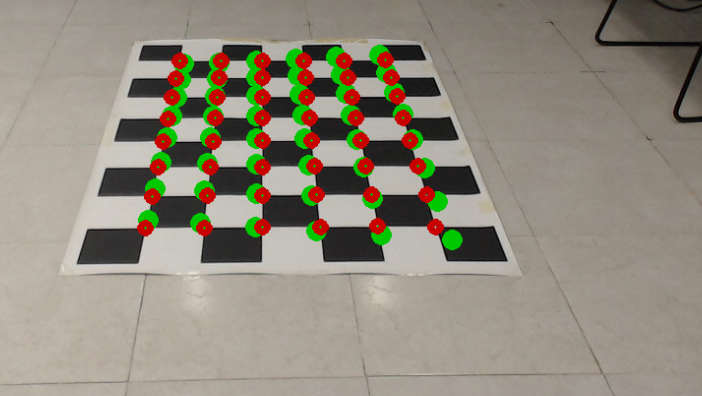
\includegraphics[width=.5\textwidth]{./pictures/conG0}
       		\caption{Reproyección de puntos}\label{fig: figura}
       	\end{figure}
       	En la figura 11.6 se puede apreciar la comparación de los puntos después de optimizar y los resultados son superiores a comparación de lo que hay antes de la optimización.
       	
       	 Sin embargo, en el último punto (esquina inferior derecha)
       	
       	\subsection{Correción de la imagen y recalibración de la cámara}
       	Como se busca que la proyección de los puntos 3d en la imagen con los puntos seleccionados sean lo más precisos posibles se recalibró la cámara (a diferentes resoluciones) con la que se realizan los experimentos mediante herramientas de OpenCV y esta vez se corrigió la distorsión de la cámara mediante los coeficientes de distorsión obtenidos de la recalibración. Todo lo anterior es con el objetivo de aumentar la precisión de la estimación de la matriz de rotación y el vector de traslación.\\
    	\begin{figure}[htbp]
    		\centering
    		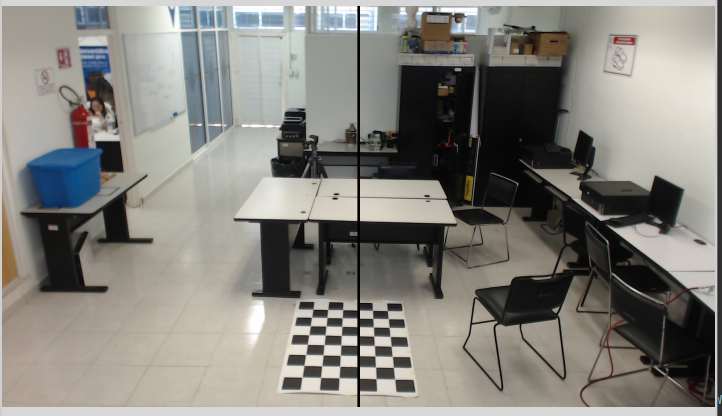
\includegraphics[width=.47\textwidth]{./pictures/p1}
    		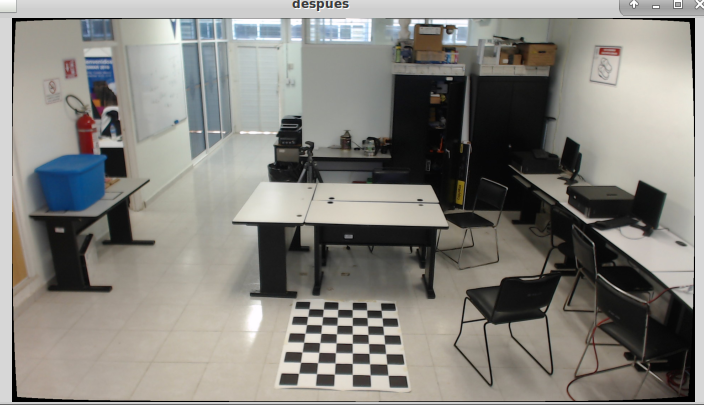
\includegraphics[width=.47\textwidth]{./pictures/p2}
    		\caption{Corrección de la imagen}\label{fig: figura}
    	\end{figure}
       	En la imagen de la izquierda de la figura 4.26 se puede apreciar la imagen antes de la corrección y en la de la derecha con la correción aplicada.\\
       	Después de aplicar lo anterior (recalibración y corrección de la cámara) y antes de optimizar se obtienen resultados muy superiores a los conseguidos hasta ahora, ya que $F(p)=  4.10149e-07$, el resultado de comparar los puntos y dibujarlos se puede apreciar en la figura \ref{correctEst}.\\
    	\begin{figure}[htbp]
    		\centering
    		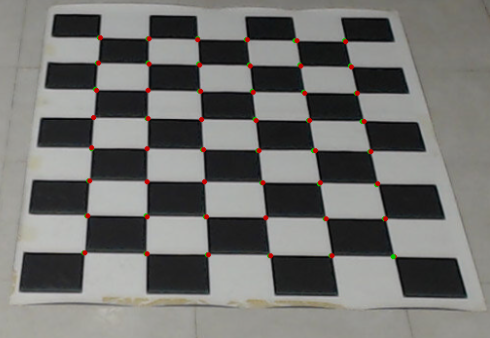
\includegraphics[width=.47\textwidth]{./pictures/correc1}
    		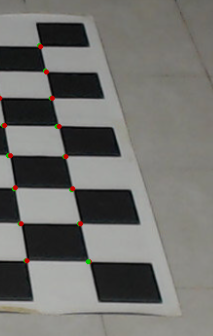
\includegraphics[width=.21\textwidth]{./pictures/correc2}
    		\caption{Estimación de R y T antes de la optimización}\label{fig: figura}
    		\label{correctEst}
    	\end{figure}
       	Aplicando nuevamente la optimización numérica a partir del resultado anterior da resultados aún mejores ya que después de 1000 iteraciones se obtiene un mínimo de  $F(p)=  2.908337e-10$ y el resultado gráfico se ve en la imagen \ref{correctEstOpt}.
       	%Colocar en el marco teórico como funciona la correción de la distorsión y la calibración
    	\begin{figure}[htbp]
    		\centering
    		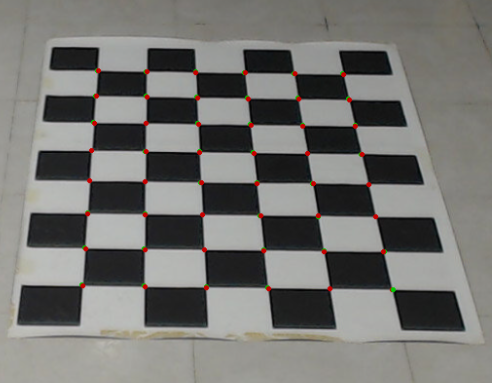
\includegraphics[width=.47\textwidth]{./pictures/correcOpt1}
    		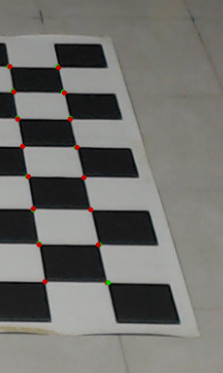
\includegraphics[width=.22\textwidth]{./pictures/correcOpt2}
    		\caption{Estimación de R y T después de la optimización p}\label{fig: figura}
    		\label{correctEstOpt}
    	\end{figure}
       	
       	
       	
       	
       	
       	
       	
       	
       	
       	
       	
       	
       	
    








 


\chapter{Resultados}

\chapter{Conclusiones}



\appendix
\chapter{Example Appendix}
Appendices are usually labelled with letters separate to ordinary chapters.



\bibliographystyle{plain}
\bibliography{referencias}
\addcontentsline{toc}{chapter}{Bibliografía}



%\bibliographystyle{plain}
%\bibliography{thesis}
%\addcontentsline{toc}{chapter}{Bibliography}
%
%\printindex
%\addcontentsline{toc}{chapter}{Index}
%
%\begin{verbatim}

%\end{verbatim}
\end{document}